\documentclass[11pt,a4paper,openany]{report}
\usepackage[T1]{fontenc}
\usepackage[utf8]{inputenc}
\usepackage{lmodern}
\usepackage{microtype}
\usepackage{amsmath,amssymb,amsthm,mathtools,bm}
\usepackage{booktabs,array,longtable,tabularx}
\usepackage{xcolor}
\usepackage[margin=24mm,headheight=23pt]{geometry}
\usepackage{enumitem}
\usepackage{fancyhdr}
\usepackage{fancyvrb}
\usepackage{graphicx}
\usepackage{url}
\usepackage{xurl}
\usepackage{hyperref}

\definecolor{finblue}{HTML}{1F5A99}
\definecolor{fingreen}{HTML}{19733A}
\definecolor{finorange}{HTML}{D55E00}
\definecolor{finred}{HTML}{A61B1B}
\definecolor{finviolet}{HTML}{6A3D9A}

\hypersetup{
  unicode=true,
  colorlinks=true,
  linkcolor=finblue,
  citecolor=fingreen,
  urlcolor=finblue,
  pdftitle={FIN Programs 138--150: State Selection, Validated Fractional Dynamics, Detector Physics, and Bridge Architecture},
  pdfauthor={Krzysztof Żuchowski},
  pdfsubject={KMS and entropy state-selection no-go theorems, validated fractional FFT, detector resolution, preparation resource theory, bridge diagram, and pre-data protocol},
  pdfkeywords={FIN, KMS states, maximum entropy, Morita equivalence, interval FFT, fractional dynamics, detector resolution, resource theory, operational physics}
}

\pagestyle{fancy}
\fancyhf{}
\fancyhead[L]{\small FIN Programs 138--150}
\fancyhead[R]{\small Release 10.14}
\fancyfoot[C]{\thepage}
\setlength{\parindent}{0pt}
\setlength{\parskip}{0.55em}
\setlist{nosep,leftmargin=2em}
\setcounter{tocdepth}{2}
\setcounter{secnumdepth}{3}
\emergencystretch=3em

\newcommand{\one}{\bm 1}
\newcommand{\C}{\mathbb C}
\newcommand{\R}{\mathbb R}
\newcommand{\Z}{\mathbb Z}
\newcommand{\statusProven}{\textcolor{fingreen}{[Proven]}}
\newcommand{\statusComputer}{\textcolor{fingreen}{[Proven, computer-assisted]}}
\newcommand{\statusStrong}{\textcolor{finblue}{[Strong evidence]}}
\newcommand{\statusConditional}{\textcolor{finorange}{[Conditional]}}
\newcommand{\statusRefuted}{\textcolor{finred}{[Refuted in scope]}}
\newcommand{\statusOpen}{\textcolor{finviolet}{[Open]}}

\begin{document}
\hypersetup{pageanchor=false}
\begin{titlepage}
\centering
\vspace*{9mm}
{\Large\bfseries FIN Research Monograph --- Release 10.14\par}
\vspace{11mm}
{\Huge\bfseries FIN Programs 138--150\par}
\vspace{6mm}
{\Large State Selection, Validated Fractional Dynamics,\\
Detector Physics, and Bridge Architecture\par}
\vspace{17mm}
{\Large Krzysztof \.Zuchowski\par}
\vspace{2mm}
{\normalsize Independent Researcher --- Fractal Information Theory Project\par}
\vspace{2mm}
{\normalsize ORCID: \href{https://orcid.org/0009-0002-0909-3613}{0009-0002-0909-3613}\par}
\vspace{10mm}
{\large 27 July 2026\par}
{\normalsize Publication --- Preprint; record version 1.0.0\par}
\vfill
\begin{minipage}{0.88\textwidth}
\small
\textbf{Scope.} Thirteen executed studies of state selection, KMS and
maximum-entropy obstructions, Morita stability, validated fractional
dynamics, detector resolution, joint system--instrument identification,
calibration-invariant observables, signed-preparation resources, completion
maps, and a frozen pre-data protocol.

\medskip
\textbf{Central result.} KMS theory, maximum entropy, and Morita equivalence
do not select the sector state producing \(9/5\). A formal interval FFT,
a reflection-asymmetry resource theorem, and a calibration-invariant
operational test are constructed.

\medskip
\textbf{Guardrail.} No canonical sector state, strict selector, internal
physical units, completed legacy--strict bridge, role transfer,
\(L_{\mathrm{total}}\), Theory-of-Everything closure, or external validation
is claimed.

\medskip
\textbf{License.} Creative Commons Attribution 4.0 International (CC BY 4.0).
\end{minipage}
\vfill
\end{titlepage}
\hypersetup{pageanchor=true}

\pagenumbering{roman}
\chapter*{Publication statement}
\addcontentsline{toc}{chapter}{Publication statement}
This release reports Programs 138--150 and recommends Programs 151--163.
Analytic proofs, formal interval certificates, conditional constructions,
synthetic evidence, falsified candidates, and open physical obligations are
kept separate.

\tableofcontents
\clearpage
\pagenumbering{arabic}

\section{Confidence convention}

The release separates the following statuses.

\begin{itemize}
\item 
\textbf{Proven:} an analytic or finite mathematical proof is supplied.

\item 
\textbf{Proven, computer-assisted:} directed interval arithmetic or a finite exhaustive computation supplies a reproducible certificate.

\item 
\textbf{Strong evidence:} a reproducible floating-point or Monte Carlo result supports a claim within a declared finite model.

\item 
\textbf{Conditional:} the result follows after an input not sourced by strict FIN is declared.

\item 
\textbf{Refuted in scope:} a candidate fails a stated necessary test.

\item 
\textbf{Open:} the required source, physical standard, or external record is absent.

\end{itemize}

A state constructed from a chosen modular Hamiltonian is not called an internally selected state. A maximum-entropy state is not called reference-free. A signed receiver is not called a source of signed preparation. Synthetic statistical power is not physical evidence.

\section{Abstract}

This monograph executes thirteen research programs addressing the three principal objects still missing between the FIN spectral core and physical testing:

\begin{enumerate}
\item 
a distinguished state on the localized sector algebra;

\item 
a nonfree preparation supplying a signed branch;

\item 
an operational detector and calibration interface.

\end{enumerate}

Programs 125--137 had produced a natural finite-carrier localizer with fibre dimensions

\[
d=(1,2,2,2,2),
\]

but found that the uniform sector state yielding

\[
\eta=\frac95
\]

was not selected by carrier naturality. The present round tests three deeper state-selection mechanisms: modular/\allowbreak{}KMS theory, maximum entropy, and Morita equivalence.

All three fail to select the uniform state without an additional premise. For the commutative sector algebra \(\mathcal A_{\mathcal F}=\mathbb C^5\), every continuous one-parameter automorphism group is trivial, so every probability state is KMS. In the noncommutative block enlargement

\[
\mathcal B
=
M_1(\mathbb C)\oplus M_2(\mathbb C)^{\oplus4},
\]

every faithful density matrix defines its own modular flow. A Gibbs family can produce \(9/5\), but only when its dimensionless modular gap is fixed to

\[
\theta=\log2=\frac{\alpha_{\rm geo}}4.
\]

No current theorem selects that gap.

Maximum relative entropy returns its reference measure. Sector counting gives \(9/5\), Hilbert microstate counting gives \(17/9\), and Hilbert--Schmidt counting gives \(33/17\). Morita-equivalent block amplifications can continuously alter the normalized Hilbert central weights. Consequently neither entropy nor Morita equivalence supplies a reference-free sector state.

The fractional analysis receives a formal proof upgrade. A radix-two interval FFT using 42-decimal-place directed interval arithmetic, together with analytic frequency-cell and tail bounds, covers every frequency in

\[
10^{-3}\le |q|\le2\cdot10^{-2}.
\]

All 50 interval cells have positive symbol lower bounds and are compatible with the \(C|q|^{4/5}\) prediction. The formal maximum relative-remainder upper bound is \(1.08135\), substantially coarser than the earlier floating-point bound of \(2.2647\%\). Thus the fractional scale is formally compatible on the full window, while the tight numerical percentage is not yet a formal theorem.

An explicit finite Diophantine modulus is also derived. The first certified continued-fraction terms of

\[
\frac{\omega}{\pi}
=
\frac{743}{4000\pi}
\]

are

\[
[0;16,1,10,2,67,2,2,5,1,2,928].
\]

Denjoy--Koksma and the Ostrowski representation give a rigorous discrepancy bound through \(N=10^6\). The large partial quotient \(928\) explains why a uniform all-scale power remainder cannot be inferred from this finite prefix.

The missing detector object is constructed in two forms. First, \(H^s(\mathbb R)\) with \(s>1/2\) supplies bounded point evaluation for fractional wave records. Second, a Gaussian response

\[
\widehat R_\sigma(q)=e^{-\sigma^2q^2/2}
\]

defines a finite-resolution measurement family. The limit \(R_\sigma U_tf\to U_tf\) exists uniformly for sufficiently regular preparations, while an ideal delta preparation has peak

\[
\frac1{\sqrt{2\pi}\sigma}
\]

and no resolution-independent limit.

A joint system--instrument inverse map separates the fractional exponent, detector error, and apparatus memory from two mean records and one lag correlation. A calibration-invariant IQR spreading statistic is then constructed:

\[
T
=
\frac{
\log\left[\operatorname{IQR}(t_2)/\operatorname{IQR}(t_1)\right]
}{
\log(t_2/t_1)
}
=\frac1\alpha.
\]

For \(\alpha=4/5\), \(T=5/4\). Multiplicative length calibration cancels.

The strongest new structural result is a preparation resource theory. Let \(R\) be reflection and define

\[
M(\rho)
=
\frac12\|\rho-R\rho R\|_1.
\]

For every reflection-covariant quantum channel \(\Phi\),

\[
M(\Phi(\rho))\le M(\rho).
\]

If \(C\) is reflection odd, then

\[
|\operatorname{Tr}(\rho C)|
\le
M(\rho)\|C\|_\infty.
\]

Therefore a reflection-symmetric state cannot generate a nonzero signed receiver under reflection-covariant operations. The missing signed preparation is a resource, not a scalar hidden in the radial kernel.

Finally, a typed completion diagram is constructed. Amplitude projectivization and conditional damping commute when the oscillatory numerator is artificially shared, with residual \(5.67\cdot10^{-17}\). For the actual canonical legacy phase/\allowbreak{}frequency \((\pi/4,\pi/6)\) and strict values, the relative residual is \(0.470865\). The phase/\allowbreak{}frequency and role-transfer arrows remain absent.

The release concludes with an immutable pre-data physical protocol distinguishing local diffusion \(\alpha=2\) from fractional spreading \(\alpha=4/5\). Its canonical core has SHA-256 0c292bf5d8efce3055a27daa16e60d60b53e2e2cb9852c37827418ec1ec453f5. No external data are admitted.

\par\medskip\hrule\medskip

\chapter{Part I --- Scope, kernel split, and fixed objects}

\section{Research objective}

Programs 138--150 answer the following questions.

\begin{enumerate}
\item 
Can modular or KMS structure select the uniform sector trace?

\item 
Does maximum entropy select that trace without a reference measure?

\item 
Is the Hilbert-trace exponent stable under Morita equivalence?

\item 
Can the continuous fractional window be enclosed by genuine interval arithmetic?

\item 
Can the irrational rotation produce an explicit finite discrepancy modulus?

\item 
Which regular wave preparations permit pointwise records?

\item 
Can detector resolution be removed, and for which preparations?

\item 
Can the generator exponent and apparatus memory be identified jointly?

\item 
Which observable ratios cancel physical calibration constants?

\item 
Can signed preparation be formalized as a resource theory?

\item 
Can one construct a coupled state--damping action without hiding \(9/5\) in its coefficients?

\item 
Which arrows in the legacy-to-strict completion diagram actually commute?

\item 
Can a physical test be frozen before external data are admitted?

\end{enumerate}

\section{Kernel split}

The canonical legacy kernel is

\[
K_{\rm legacy}(d)
=
\alpha_{\rm geo}
\frac{\cos\left(\frac\pi4d+\frac\pi6\right)}
{1+\beta_{\rm tors}d},
\qquad
\beta_{\rm tors}=0.01.
\]

The strict working kernel is

\[
K_{\rm strict}(d)
=
\frac{\cos(\omega_sd+\phi_s)}
{1+d^{9/5}},
\]

where

\[
\omega_s=\frac{743}{4000},
\qquad
\phi_s=\frac{13}{80}.
\]

The legacy kernel remains an intermediate bridge object. The strict kernel is a later gate-selected working kernel. A map that corrects only amplitude or damping does not identify their oscillatory numerators.

\section{Localized sector algebra}

The finite-carrier localizer is

\[
\mathcal F_p
=
\widetilde H_0(\ker m_p)
\oplus\mathcal X_p^-,
\]

with

\[
\dim\mathcal F_p=(1,2,2,2,2)
\]

for \(p=2,3,5,7,11\). The associated center is

\[
\mathcal A_{\mathcal F}=\mathbb C^5.
\]

A state on this center is a probability vector \(w\). The exponent readout is

\[
\eta(w)=\sum_pw_p\dim\mathcal F_p=2-w_2.
\]

The localizer is natural. The state is not yet selected.

\section{Fractional generator}

For stochastic and continuum calculations, use

\[
a_d=
\frac{|\cos(\omega_sd+\phi_s)|}{1+d^{9/5}},
\qquad
p_{\pm d}=\frac{a_d}{2\sum_{j\ge1}a_j}.
\]

The symbol is

\[
S(q)=1-\widehat p(q),
\]

and its candidate small-frequency law is

\[
S(q)\sim C|q|^{4/5}.
\]

The continuum generator is

\[
A=C(-\Delta)^{2/5}.
\]

This dimensionless generator does not itself define physical units, preparation, detector resolution, or an external record.

\par\medskip\hrule\medskip

\chapter{Part II --- Programs 138--140: three state-selection no-go theorems}

\section{Program 138 --- Modular and KMS selection}

\subsection{Commutative obstruction}

The automorphism group of \(\mathbb C^5\) is the finite permutation group \(S_5\). A continuous homomorphism

\[
\alpha:\mathbb R\to S_5
\]

must be constant because \(\mathbb R\) is connected and \(S_5\) is discrete. Therefore every continuous one-parameter automorphism group of \(\mathbb C^5\) is trivial.

For trivial dynamics, the KMS relation reduces to commutativity. Every probability state on \(\mathbb C^5\) is KMS for every inverse temperature.

\textbf{Theorem 138.1:} KMS on the commutative sector algebra does not select a state.

\subsection{Noncommutative enlargement}

Use the fibre dimensions to form

\[
\mathcal B
=
M_1(\mathbb C)
\oplus
M_2(\mathbb C)^{\oplus4}.
\]

For every faithful density \(\rho\),

\[
\sigma_t^\rho(a)
=
\rho^{it}a\rho^{-it}
\]

is a modular flow and \(\rho\) is KMS for that flow. Modular theory therefore relates a state to a flow; it does not choose the state before the flow or density is supplied.

\subsection{Intrinsic block-Gibbs family}

Assign energy zero to the one-dimensional block and a common gap \(\Delta\) to the four two-dimensional blocks. With

\[
\theta=\beta\Delta,
\]

the central weight of the exceptional block is

\[
w_2(\theta)
=
\frac1{1+8e^{-\theta}},
\]

and

\[
\eta(\theta)=2-w_2(\theta).
\]

At \(\theta=0\), this is the normalized Hilbert state and

\[
\eta(0)=\frac{17}{9}.
\]

The target value occurs only at

\[
\eta=\frac95
\quad\Longleftrightarrow\quad
\theta=\log2=\frac{\alpha_{\rm geo}}4.
\]

\begin{figure}[htbp]
\centering
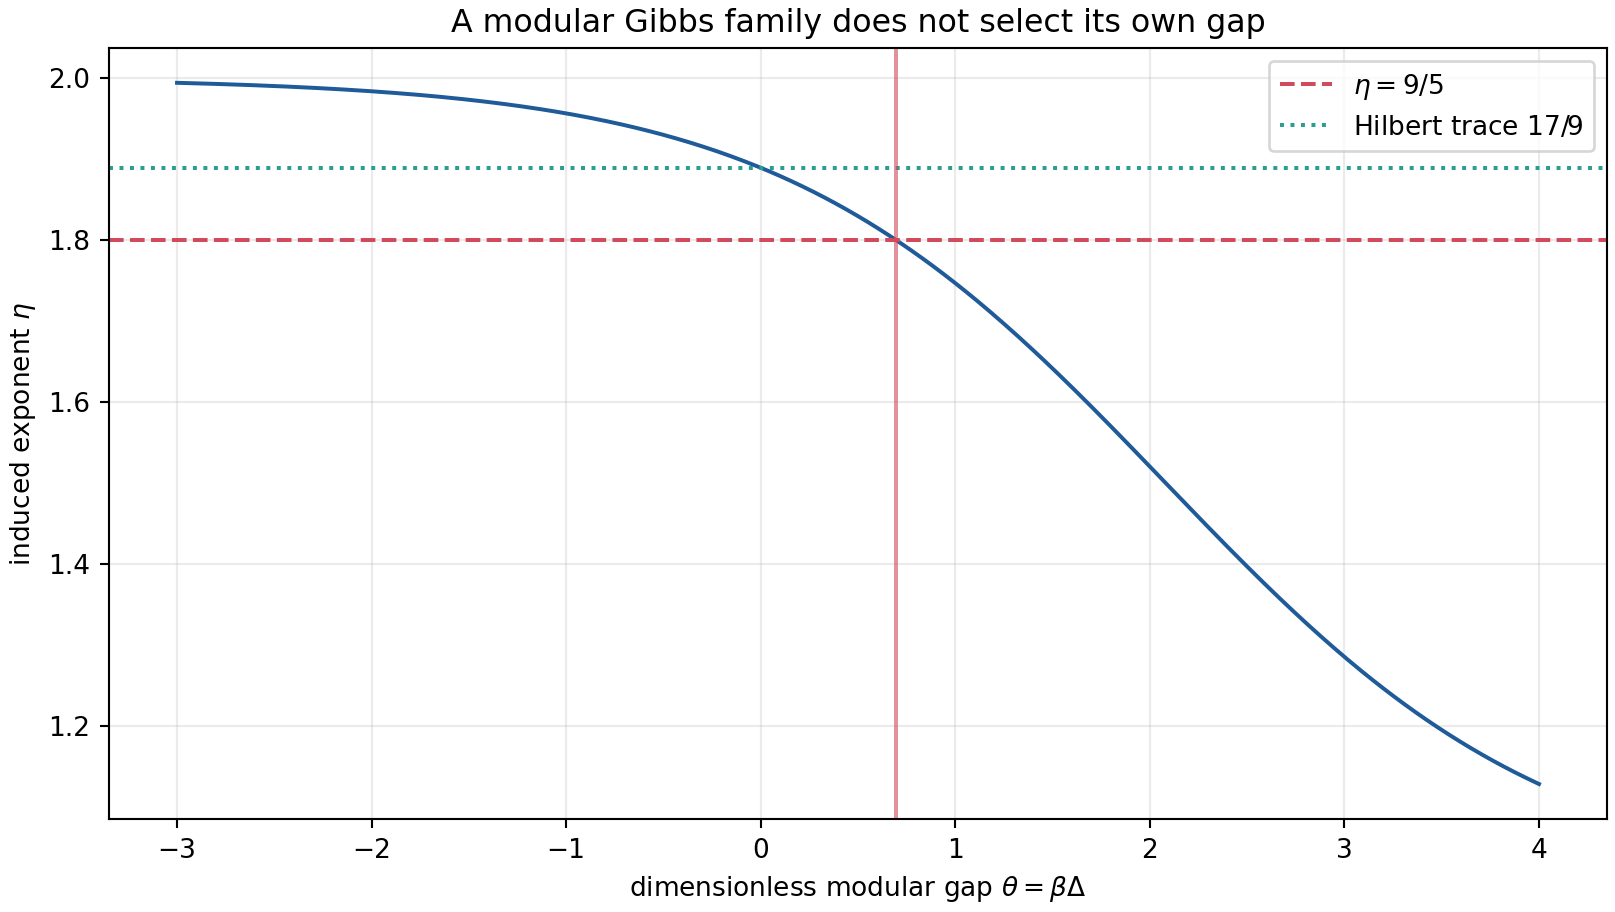
\includegraphics[width=0.94\textwidth]{FIN_Programs_138_150_State_Detector_Bridge_Figures/program138_modular_kms_family.png}
\caption{The block-Gibbs modular family realizes \(9/5\) only after a gap \(\theta=\log 2\) is supplied.}
\end{figure}

\textbf{Result:} \textbf{Proven.} A chosen modular gap realizes \(9/5\), but modular theory does not source the gap.

\textbf{Falsification boundary:} writing \(\theta=\alpha_{\rm geo}/4\) is an exact identity after \(\theta\) is chosen. It is not a derivation of why the modular Hamiltonian must have that gap.

\section{Program 139 --- Maximum entropy and the reference measure}

Let \(r\) be a faithful reference state. Maximizing negative relative entropy,

\[
-D(w\|r),
\]

without other constraints has the unique solution

\[
w=r.
\]

The conclusion of maximum entropy therefore depends on the declared sample space.

\subsection{Three natural-looking references}

For

\[
r_{a,p}
\propto
d_p^a,
\]

three choices give:

\[
\begin{array}{c|c|c}
a & \text{interpretation} & \eta\\
\hline
0 & \text{sector counting} & 9/5\\
1 & \text{Hilbert microstate counting} & 17/9\\
2 & \text{Hilbert--Schmidt counting} & 33/17.
\end{array}
\]

All are mathematically legitimate. None is selected by entropy alone.

\begin{figure}[htbp]
\centering
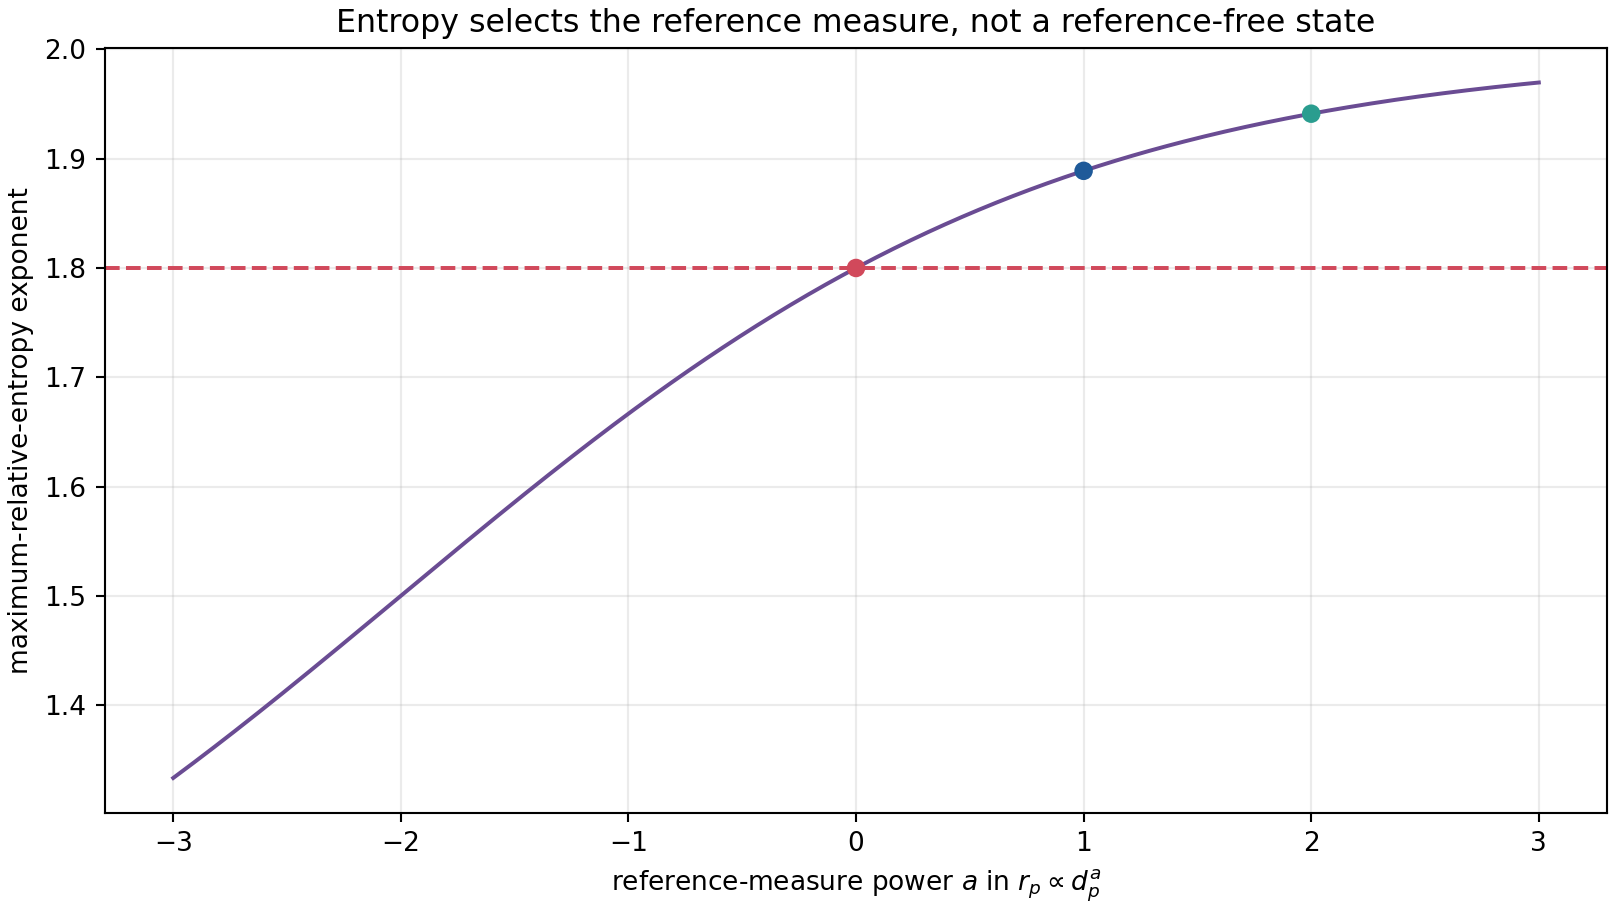
\includegraphics[width=0.94\textwidth]{FIN_Programs_138_150_State_Detector_Bridge_Figures/program139_entropy_reference_classification.png}
\caption{Maximum relative entropy returns the chosen reference measure.}
\end{figure}

\subsection{Constraint circularity}

Imposing

\[
\sum_pw_pd_p=\frac95
\]

is exactly equivalent to imposing \(w_2=1/5\). Entropy can then distribute the remaining weights, but the desired exponent already appears in the constraint.

Full \(S_5\) symmetry would force equal sector weights, but it exchanges the one-dimensional and two-dimensional fibre blocks. It is not a symmetry of the localized block structure.

\textbf{Result:} \textbf{Proven.} Uniform maximum entropy is conditional on sector counting or an equivalent constraint. No reference-free entropy theorem is obtained.

\section{Program 140 --- Morita stability}

Consider block amplifications

\[
\mathcal B_{\mathbf n}
=
\bigoplus_p M_{n_pd_p}(\mathbb C).
\]

Each is strongly Morita equivalent to \(\mathbb C^5\). Its normalized full Hilbert trace induces central weights

\[
w_p(\mathbf n)
=
\frac{n_pd_p}{\sum_qn_qd_q}.
\]

For the original blocks \(\mathbf n=(1,1,1,1,1)\),

\[
\eta=\frac{17}{9}.
\]

For \(\mathbf n=(2,1,1,1,1)\), all central weights are equal and

\[
\eta=\frac95.
\]

For \(\mathbf n=(20,1,1,1,1)\),

\[
\eta=\frac97\approx1.285714.
\]

Blockwise amplification therefore changes the Hilbert-trace exponent while preserving Morita equivalence.

\begin{figure}[htbp]
\centering
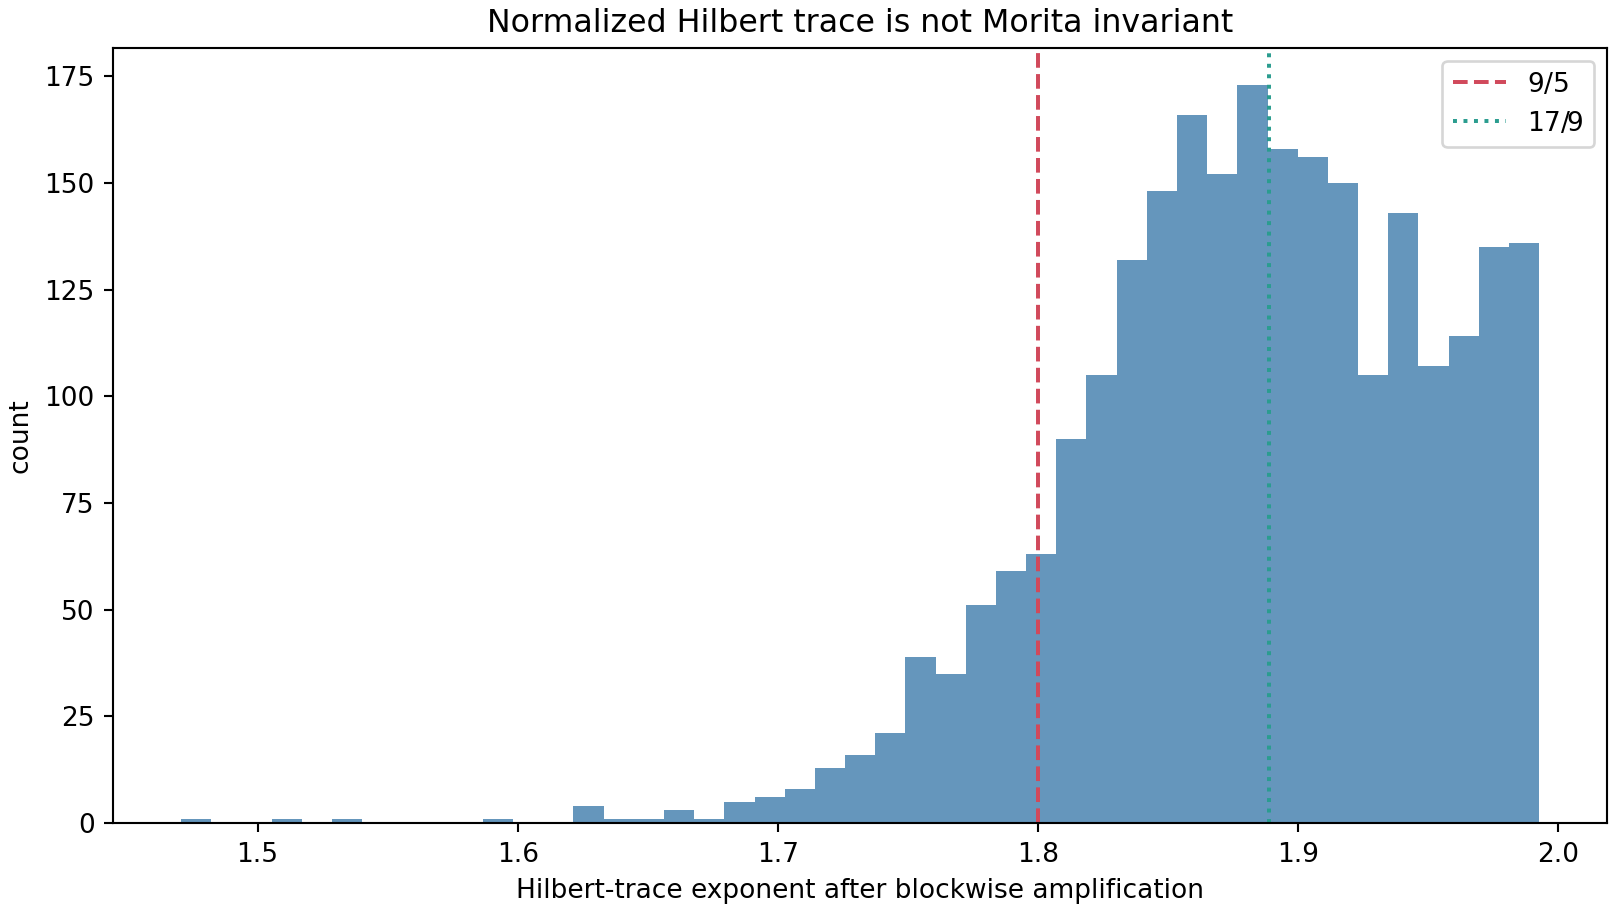
\includegraphics[width=0.94\textwidth]{FIN_Programs_138_150_State_Detector_Bridge_Figures/program140_morita_amplification.png}
\caption{Morita-equivalent block amplifications change normalized Hilbert central weights.}
\end{figure}

\textbf{Result:} \textbf{Proven.} Morita equivalence preserves the center up to isomorphism but does not select a probability state on that center.

\section{Integrated state-selection theorem}

The three programs imply:

\begin{quote}\itshape
The current localized finite object does not contain a canonical state selected by modularity, entropy, or Morita equivalence. Each method becomes selective only after a modular Hamiltonian, reference measure, constraint, or representation multiplicity is supplied.

\end{quote}

The missing object is therefore a state-selection law, not another re-expression of the dimension vector.

\par\medskip\hrule\medskip

\chapter{Part III --- Programs 141--142: formal fractional certification}

\section{Program 141 --- Validated interval FFT}

\subsection{Construction}

A radix-two FFT of length

\[
N=2^{14}=16384
\]

was implemented with mpmath.iv interval complex arithmetic at 42 decimal digits. The input weights, twiddle factors, butterfly operations, Fourier values, normalization, and Abelian constant are all enclosed.

Distances through

\[
D=8191
\]

are retained. The omitted normalization obeys

\[
2\sum_{d>D}d^{-9/5}
\le0.001850420657.
\]

For every Fourier cell, the variation between its center and any point in the cell is bounded by

\[
\delta q\,
2\sum_{d=1}^D d a_d.
\]

\subsection{Certificate}

Fifty cells cover exactly

\[
[0.001,0.02].
\]

The Abelian constant is enclosed by

\[
C\in[1.1470611724,1.1481405095].
\]

Every symbol lower bound is positive, and every cell is compatible with the fractional prediction. The worst cell is the first one:

\[
q\in[0.001,0.0013422332],
\]

\[
S(q)\in[0.00138437,0.00950453],
\]

while

\[
Cq^{4/5}\in[0.00456653,0.00578439].
\]

The maximum formal relative-remainder upper bound is

\[
1.08134524.
\]

\begin{figure}[htbp]
\centering
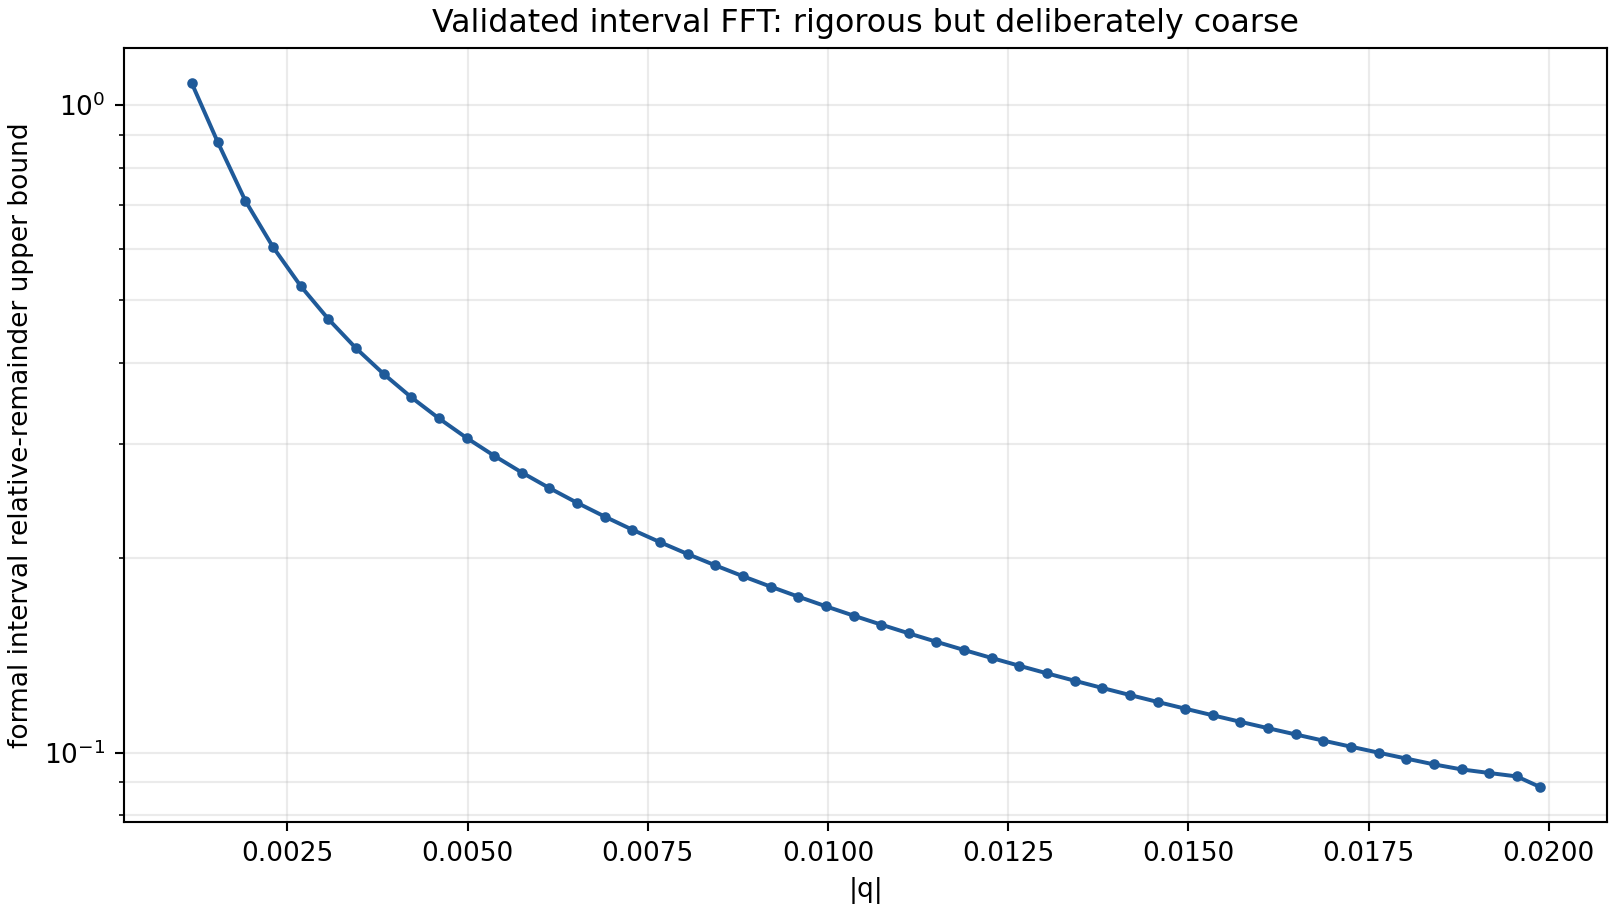
\includegraphics[width=0.94\textwidth]{FIN_Programs_138_150_State_Detector_Bridge_Figures/program141_validated_interval_fft.png}
\caption{Formal interval-FFT remainder bounds on every frequency cell in the declared window.}
\end{figure}

\textbf{Result:} \textbf{Proven, computer-assisted.} The full frequency window has a formal interval enclosure compatible with the fractional scale.

\textbf{Negative result:} the tight \(2.2647\%\) floating-point bound from Program 127 is not formally recovered. The interval tail at \(D=8191\) is too large at the lowest frequency.

This distinction is scientifically important:

\begin{itemize}
\item 
formal but coarse: established here;

\item 
tight but guarded floating point: established in Program 127;

\item 
formal and tight: still open.

\end{itemize}

\section{Program 142 --- Finite Diophantine discrepancy}

\subsection{Certified continued fraction}

Directed interval arithmetic certifies

\[
\frac{743}{4000\pi}
=
[0;16,1,10,2,67,2,2,5,1,2,928,\ldots].
\]

The associated denominator sequence begins

\[
1,\ 16,\ 17,\ 186,\ 389,\ 26249,\ 52887,\ 132023,\
713002,\ 845025,\ 2403052,\ldots
\]

\subsection{Denjoy--Koksma/\allowbreak{}Ostrowski bound}

For

\[
f(x)=|\cos(\pi x+\phi)|,
\]

the total variation on the circle is \(2\). If

\[
N=\sum_jb_jq_j
\]

is the Ostrowski expansion relative to the certified rotation, then

\[
\left|
\sum_{d=1}^N f(x+d\theta)
-N\int_0^1f
\right|
\le
2\sum_jb_j.
\]

This gives an explicit theorem for every \(N\le10^6\). At \(N=10^6\), the formal absolute discrepancy bound is \(124\). The observed discrepancy is \(0.313828\), well inside the theorem bound.

\begin{figure}[htbp]
\centering
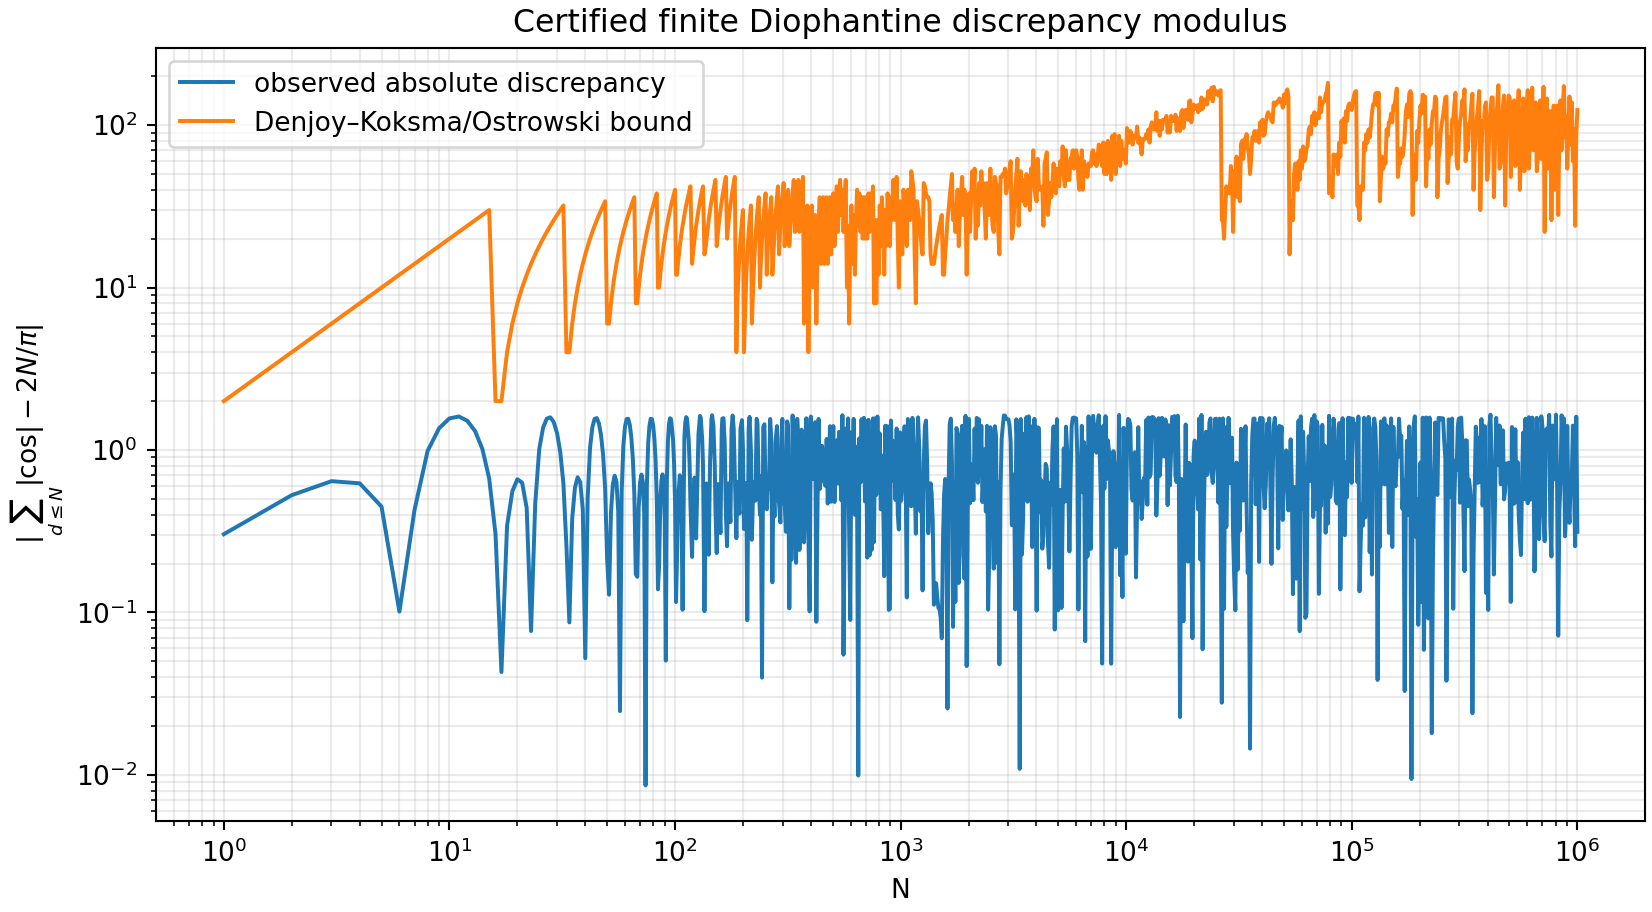
\includegraphics[width=0.94\textwidth]{FIN_Programs_138_150_State_Detector_Bridge_Figures/program142_diophantine_discrepancy.png}
\caption{The finite Denjoy--Koksma/Ostrowski discrepancy modulus and observed discrepancy.}
\end{figure}

\subsection{All-scale obstruction}

The partial quotients \(67\) and \(928\) show that the rotation is not behaving like a uniformly bounded-type number over the certified range. A finite continued-fraction prefix cannot constrain every future partial quotient. Therefore no all-scale estimate

\[
|R(q)|\le C|q|^{4/5+\delta}
\]

with fixed \(\delta>0\) follows from this finite certificate.

\textbf{Result:} \textbf{Proven finite discrepancy theorem; all-scale rate open.}

\par\medskip\hrule\medskip

\chapter{Part IV --- Programs 143--146: detector physics and identifiable observables}

\section{Program 143 --- Weighted fractional-wave records}

The unitary group

\[
U_t=e^{-itC(-\Delta)^{2/5}}
\]

preserves every Sobolev norm:

\[
\|U_tf\|_{H^s}=\|f\|_{H^s}.
\]

In one dimension, point evaluation is bounded for \(s>1/2\). By Cauchy--Schwarz,

\[
|U_tf(x)|
\le
C_s\|f\|_{H^s},
\]

where

\[
C_s^2
=
\frac1{2\pi}
\int_{\mathbb R}(1+q^2)^{-s}\,dq
=
\frac1{2\sqrt\pi}
\frac{\Gamma(s-\tfrac12)}{\Gamma(s)}.
\]

The constant diverges as \(s\downarrow1/2\).

\begin{figure}[htbp]
\centering
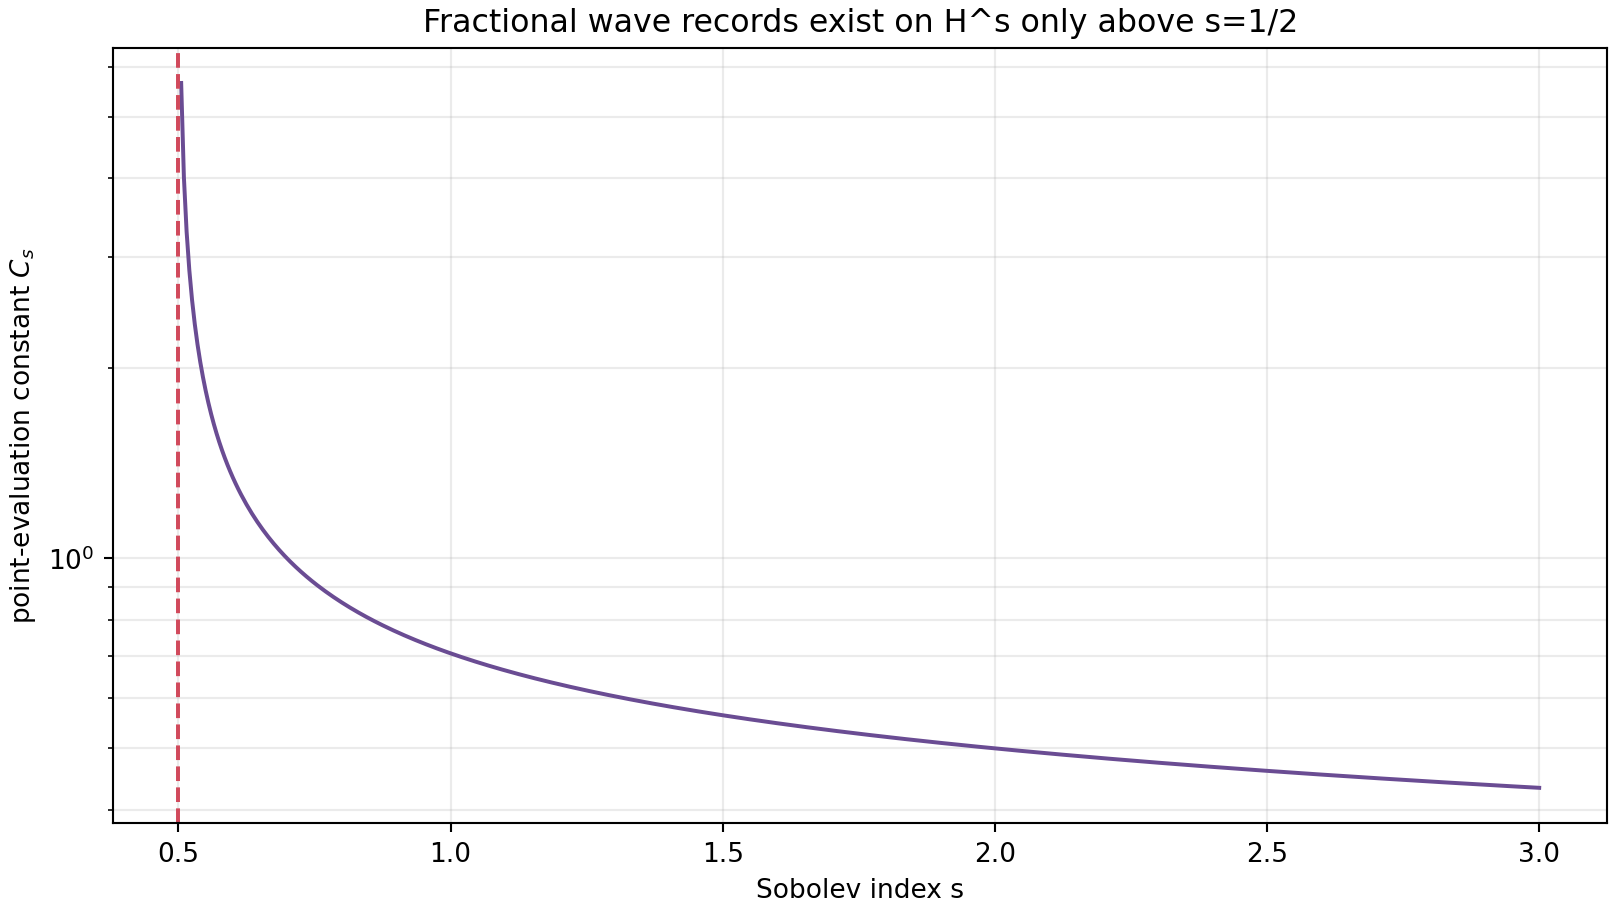
\includegraphics[width=0.94\textwidth]{FIN_Programs_138_150_State_Detector_Bridge_Figures/program143_weighted_wave_estimates.png}
\caption{The Sobolev point-evaluation constant diverges as \(s\) approaches \(1/2\).}
\end{figure}

\textbf{Result:} \textbf{Proven.} Regular preparations in \(H^s\), \(s>1/2\), define pointwise wave records.

\textbf{Limitation:} the wave group is unitary and does not smooth. This theorem does not recover an \(L^1\to L^\infty\) dispersive decay estimate and does not select a physical preparation regularity.

\section{Program 144 --- Detector-resolution renormalization}

Define a Gaussian detector response

\[
\widehat R_\sigma(q)
=
e^{-\sigma^2q^2/2}
\]

and the measured wave operator

\[
\mathcal M_{\sigma,t}=R_\sigma U_t.
\]

For \(1/2<s<5/2\),

\[
\|(R_\sigma-I)U_tf\|_\infty
\le
C_s\sigma^{s-1/2}\|f\|_{H^s}.
\]

Thus sufficiently regular preparations have a resolution-independent pointwise limit.

For the smooth test preparation

\[
\widehat f(q)=e^{-q^2/2},
\]

the observed small-\(\sigma\) error scales numerically as

\[
\sigma^{1.99924}.
\]

In contrast, an ideal delta preparation at \(t=0\) produces detector peak

\[
(R_\sigma\delta)(0)
=
\frac1{\sqrt{2\pi}\sigma},
\]

which diverges.

\begin{figure}[htbp]
\centering
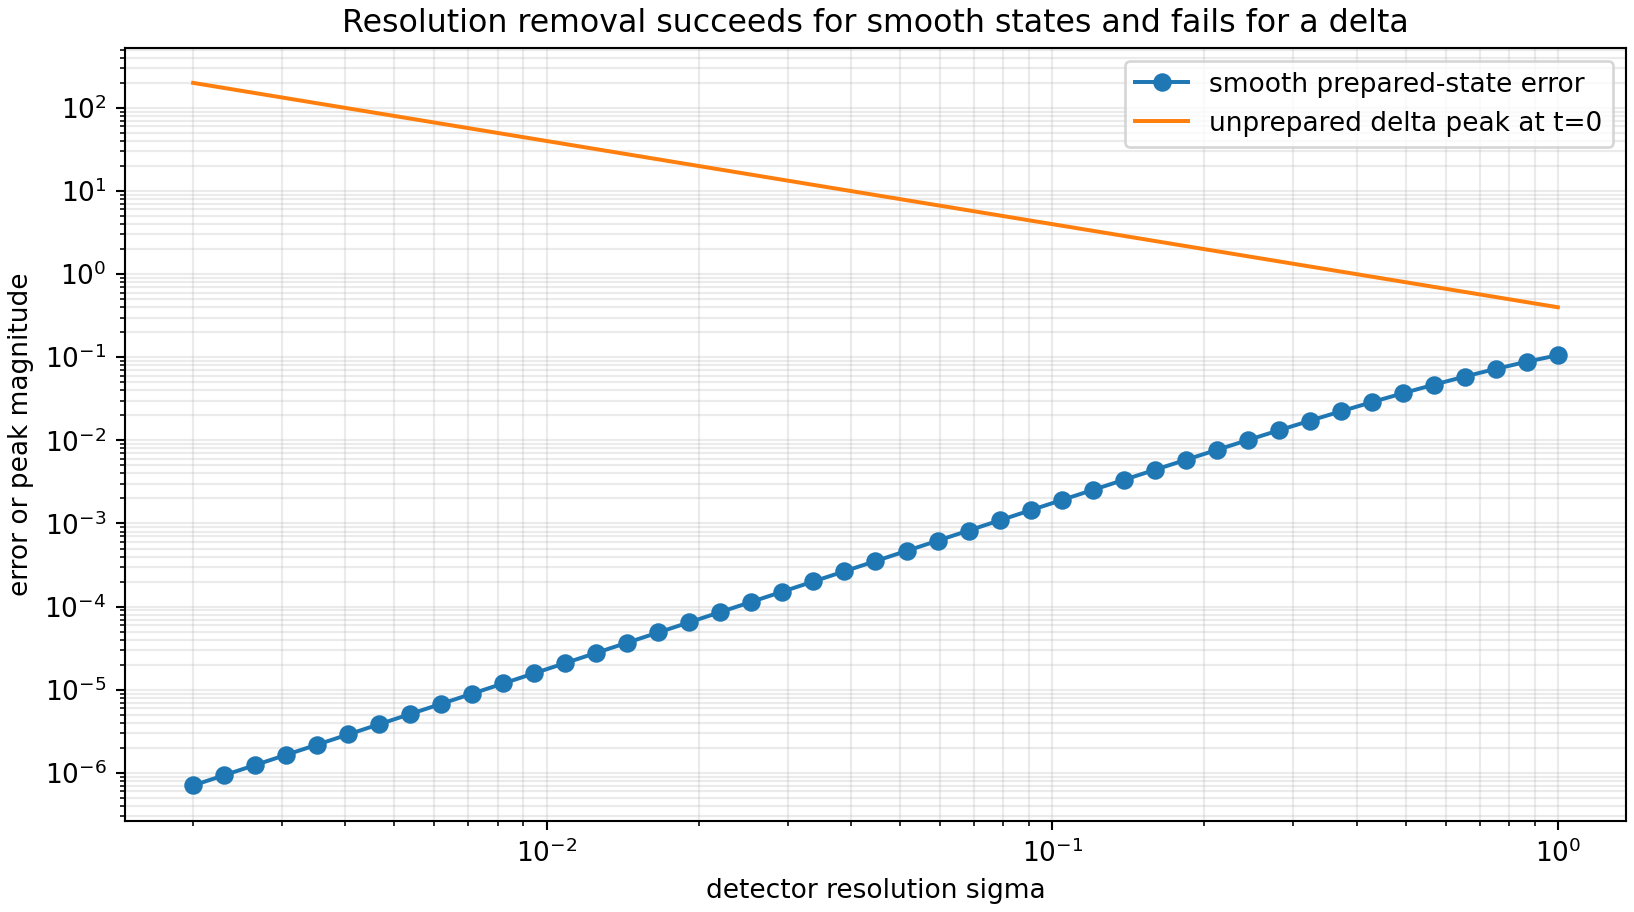
\includegraphics[width=0.94\textwidth]{FIN_Programs_138_150_State_Detector_Bridge_Figures/program144_detector_resolution.png}
\caption{Resolution removal succeeds for a smooth preparation and fails for an ideal delta.}
\end{figure}

\textbf{Result:} \textbf{Proven conditionally on preparation regularity, with a numerical rate check.}

The missing detector object can therefore be supplied without a hard cutoff, but the ability to remove its resolution depends on the preparation class.

\section{Program 145 --- Joint system--instrument identifiability}

\subsection{Declared model}

Let the system spin mean be

\[
s_\alpha(t)=e^{-t^\alpha}.
\]

Let the apparatus flip process have prevalence \(\epsilon\), signed mean

\[
e=1-2\epsilon,
\]

and persistence \(\rho\). Use the observables

\[
\mu_1=e\,s_\alpha(1),
\qquad
\mu_2=e\,s_\alpha(2),
\]

and the lag product

\[
L=s_\alpha(1)s_\alpha(2)
\left[e^2+\rho(1-e^2)\right].
\]

\subsection{Exact inverse}

The exponent is recovered from the ratio:

\[
\alpha
=
\log_2\left(
1+\log\frac{\mu_1}{\mu_2}
\right).
\]

Then

\[
e=\frac{\mu_1}{e^{-1}},
\qquad
\epsilon=\frac{1-e}{2},
\]

and

\[
\rho
=
\frac{
L/[s_\alpha(1)s_\alpha(2)]-e^2
}{
1-e^2
}.
\]

The three-observable Jacobian has rank three. A single-time mean has rank one.

At truth

\[
(\alpha,\epsilon,\rho)=(0.8,0.1,0.75),
\]

synthetic inversion with observable noise \(2\cdot10^{-4}\) gives RMSE

\[
(0.001284,\ 0.000277,\ 0.009423).
\]

\begin{figure}[htbp]
\centering
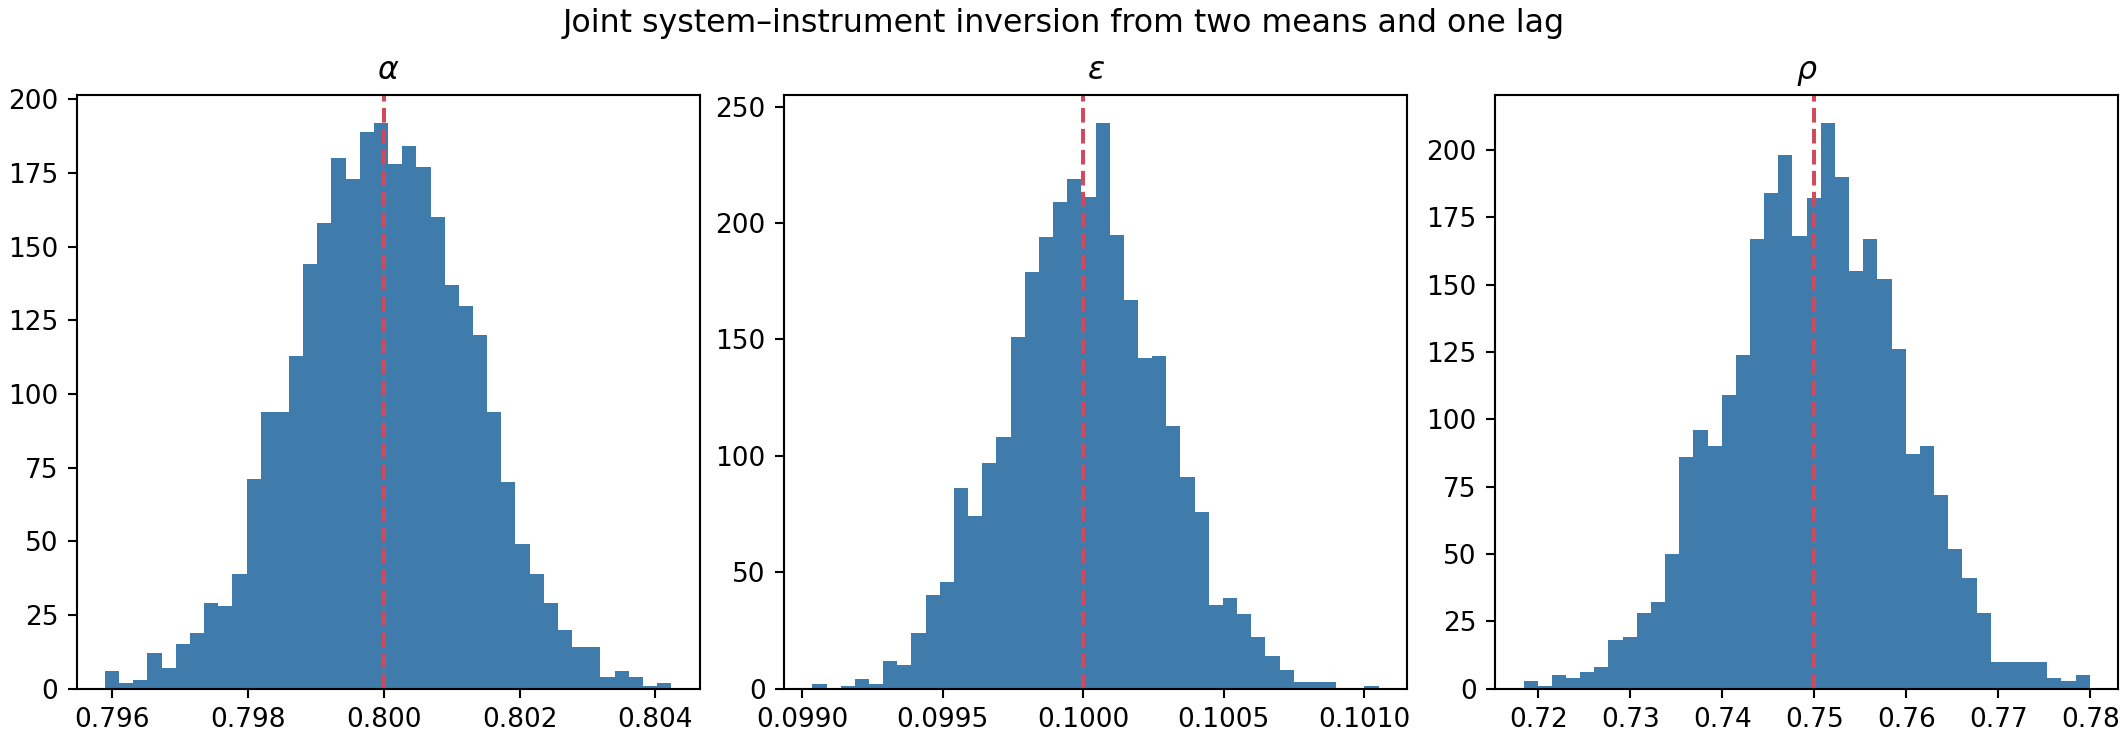
\includegraphics[width=0.94\textwidth]{FIN_Programs_138_150_State_Detector_Bridge_Figures/program145_joint_identifiability.png}
\caption{Joint inversion of fractional exponent, detector error, and apparatus memory.}
\end{figure}

\textbf{Result:} \textbf{Proven in the declared three-parameter model and validated synthetically.}

The theorem shows that memory need not be confused with a fractional exponent when two times and one correlation are measured. It is not a universal semiparametric identifiability theorem.

\section{Program 146 --- Calibration-invariant observables}

For a symmetric stable process of index \(\alpha\),

\[
X_t\overset d=t^{1/\alpha}X_1.
\]

Therefore every fixed quantile width obeys

\[
Q(t)=\ell\left(\frac{t_{\rm phys}}{\tau}\right)^{1/\alpha}Q(1).
\]

The ratio statistic

\[
T
=
\frac{
\log[Q(t_2)/Q(t_1)]
}{
\log(t_2/t_1)
}
\]

cancels \(\ell\) and \(\tau\) and equals \(1/\alpha\).

For IQR, \(t_1=1\), \(t_2=4\), and \(\alpha=4/5\), 350 synthetic replicates with 4,000 records per time give

\[
\overline T=1.25065,\qquad
\operatorname{sd}(T)=0.03147.
\]

After relative Gaussian detector noise \(0.1\ell\),

\[
\overline T=1.24799,\qquad
\operatorname{sd}(T)=0.03163.
\]

\begin{figure}[htbp]
\centering
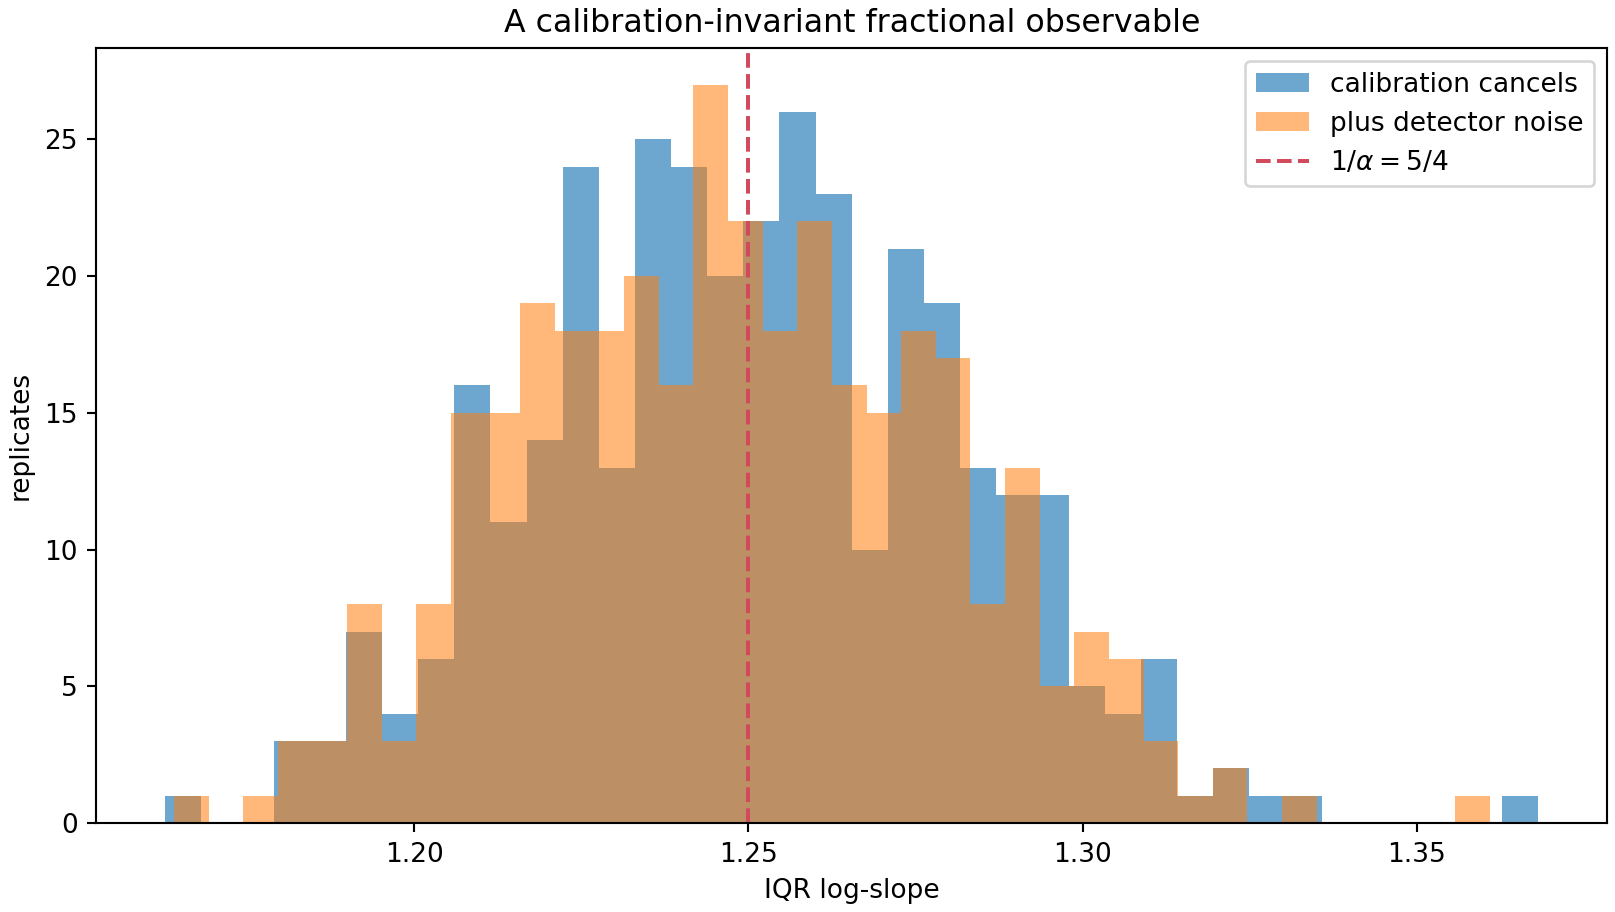
\includegraphics[width=0.94\textwidth]{FIN_Programs_138_150_State_Detector_Bridge_Figures/program146_calibration_invariant_ratio.png}
\caption{The IQR log-slope cancels multiplicative calibration and estimates the stable scaling exponent.}
\end{figure}

Other invariant candidates include spectral gap ratios,

\[
\frac{\Delta E_k}{\Delta E_j}
=
\frac{\lambda_k}{\lambda_j},
\]

which cancel \(\hbar/\tau\).

\textbf{Result:} \textbf{Constructed, with strong synthetic evidence.}

Multiplicative scales cancel, but calibrated time ordering and a detector model remain necessary.

\par\medskip\hrule\medskip

\chapter{Part V --- Programs 147--149: resource theory, action, and bridge diagram}

\section{Program 147 --- Reflection-asymmetry preparation resource}

\subsection{Free objects}

Let \(R\) implement reflection on \(C_{12}\). Define free states by

\[
\rho=R\rho R
\]

and free channels by reflection covariance,

\[
\Phi(R\rho R)=R\Phi(\rho)R.
\]

\subsection{Resource monotone}

Define

\[
M(\rho)
=
\frac12\|\rho-R\rho R\|_1.
\]

Trace-norm contractivity gives

\[
M(\Phi(\rho))
\le
M(\rho).
\]

This is a resource monotone for signed preparation.

\subsection{Receiver bound}

For any Hermitian reflection-odd receiver \(C\),

\[
RCR=-C.
\]

Then

\[
\operatorname{Tr}(\rho C)
=
\frac12
\operatorname{Tr}\left[
(\rho-R\rho R)C
\right],
\]

so Hölder duality gives

\[
|\operatorname{Tr}(\rho C)|
\le
M(\rho)\|C\|_\infty.
\]

On the fractional \(C_{12}\) circulant, the \(k=\pm1\) states satisfy

\[
M(\rho_\pm)=1,
\]

\[
\Lambda(\rho_+)=+0.498004,
\qquad
\Lambda(\rho_-)=-0.498004.
\]

Their equal mixture has

\[
M\left(\frac{\rho_++\rho_-}{2}\right)=0
\]

and zero signed receiver.

\begin{figure}[htbp]
\centering
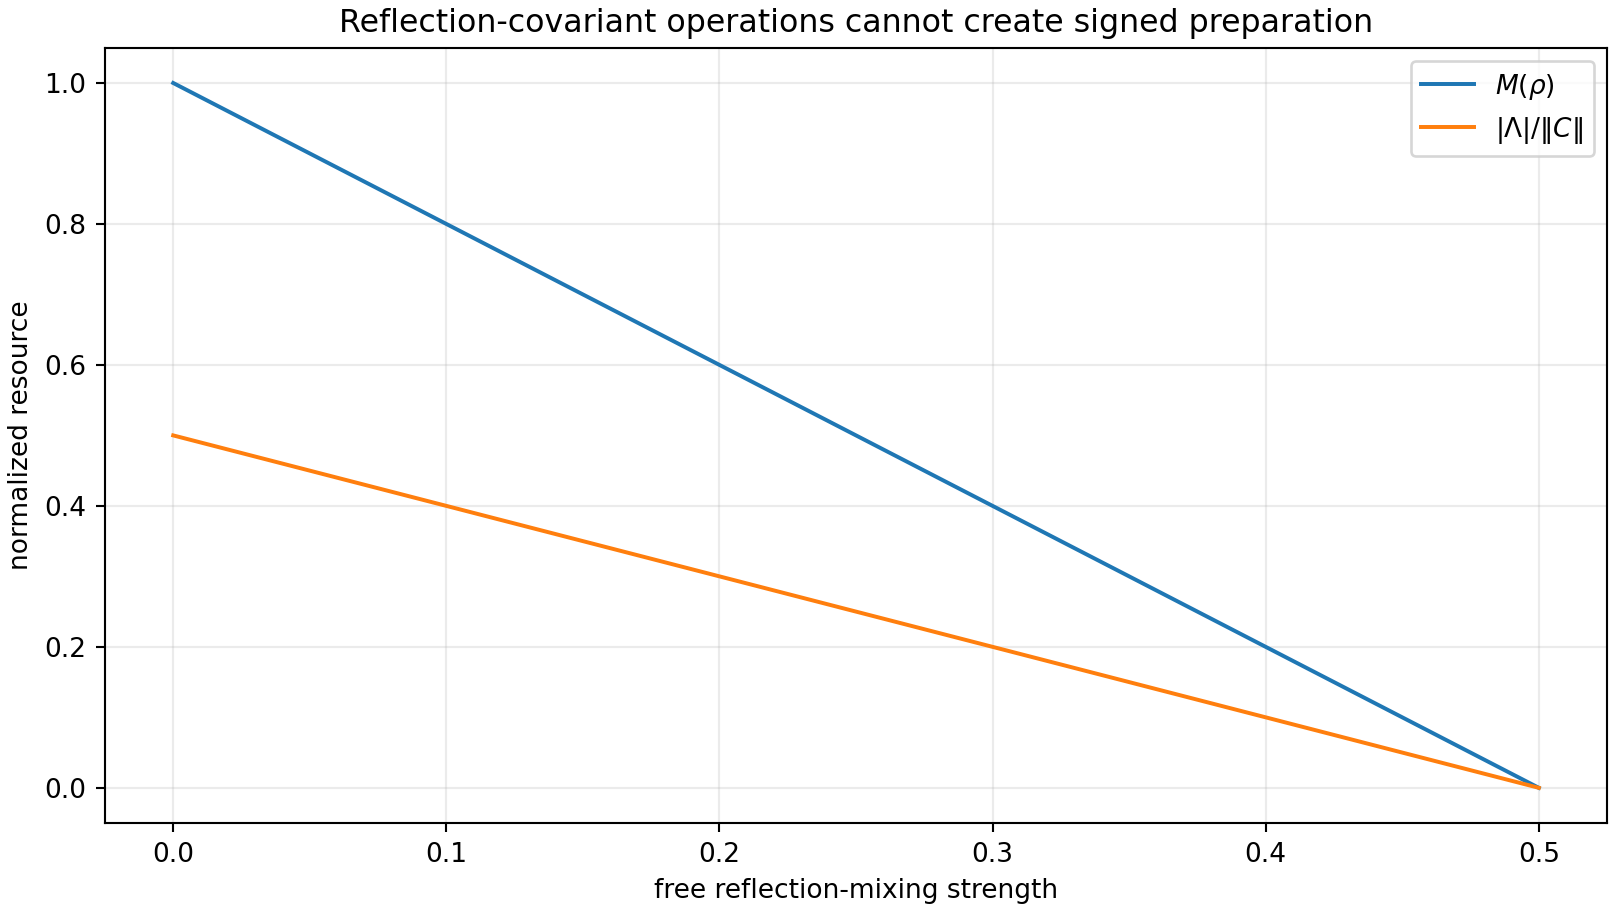
\includegraphics[width=0.94\textwidth]{FIN_Programs_138_150_State_Detector_Bridge_Figures/program147_preparation_resource.png}
\caption{Reflection-covariant operations monotonically destroy rather than create signed preparation.}
\end{figure}

\textbf{Result:} \textbf{Proven preparation-resource no-go theorem.}

A reflection-symmetric state cannot produce signed preparation under reflection-covariant operations. To discharge QW-2191, strict FIN would have to export a nonfree state or a symmetry-breaking operation. The radial kernel and even fractional generator cannot do so alone.

\section{Program 148 --- Coupled state--damping variational family}

Define

\[
r_{a,p}
=
\frac{d_p^a}{\sum_qd_q^a}
\]

and, for \(\kappa>0\),

\[
\mathcal F_{a,\kappa}(w,\eta)
=
D_{\rm KL}(w\|r_a)
+
\frac\kappa2
\left(
\eta-\sum_pw_pd_p
\right)^2.
\]

The functional is strictly convex on the simplex interior times \(\mathbb R\). Its unique stationary solution is

\[
w=r_a,
\qquad
\eta=\sum_pr_{a,p}d_p.
\]

For \(a=0\),

\[
\eta=\frac95.
\]

For \(a=1\),

\[
\eta=\frac{17}{9}.
\]

\begin{figure}[htbp]
\centering
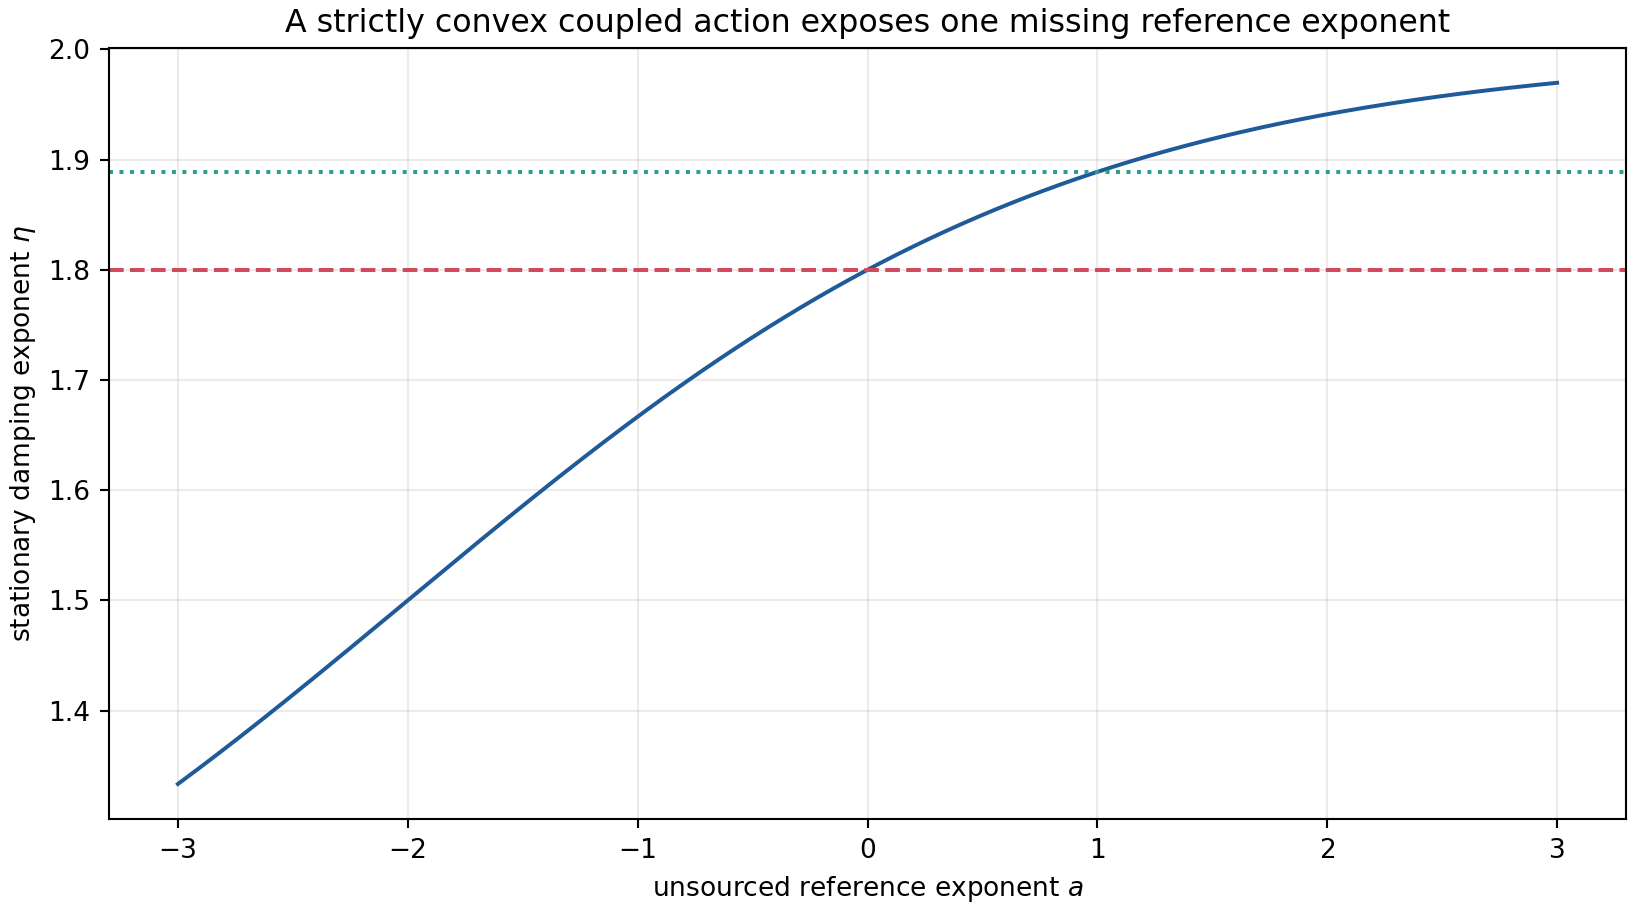
\includegraphics[width=0.94\textwidth]{FIN_Programs_138_150_State_Detector_Bridge_Figures/program148_coupled_variational_family.png}
\caption{The coupled state--damping action exposes one unsourced reference exponent.}
\end{figure}

The positive monomial tail condition

\[
T(ab)=T(a)T(b),
\qquad
T(d)=\beta d^\eta
\]

still forces \(\beta=1\) separately.

\textbf{Result:} \textbf{Constructed well-posed variational family.}

The action does not solve state selection: it exposes the remaining missing coefficient as the reference exponent \(a\). Choosing \(a=0\) because it yields \(9/5\) would be target coding.

\section{Program 149 --- Typed completion-map diagram}

\subsection{Proven and conditional arrows}

Amplitude projectivization is

\[
\Pi_0(K)=\frac{K}{K(0)}.
\]

The conditional damping multiplier is

\[
D(d)
=
\frac{1+\beta_{\rm tors}d}{1+d^{9/5}}.
\]

If the legacy oscillatory numerator is artificially replaced by the strict one, the square

\[
\Pi_0
\quad\text{followed by}\quad
D
\]

commutes with the projective strict target. The numerical residual is

\[
5.67\cdot10^{-17}.
\]

\subsection{Actual canonical parameters}

For the canonical legacy numerator

\[
\cos\left(\frac\pi4d+\frac\pi6\right)
\]

and strict numerator

\[
\cos\left(\frac{743}{4000}d+\frac{13}{80}\right),
\]

the same amplitude-plus-damping route has relative residual

\[
0.47086477
\]

on \(d=0,\ldots,64\).

\begin{figure}[htbp]
\centering
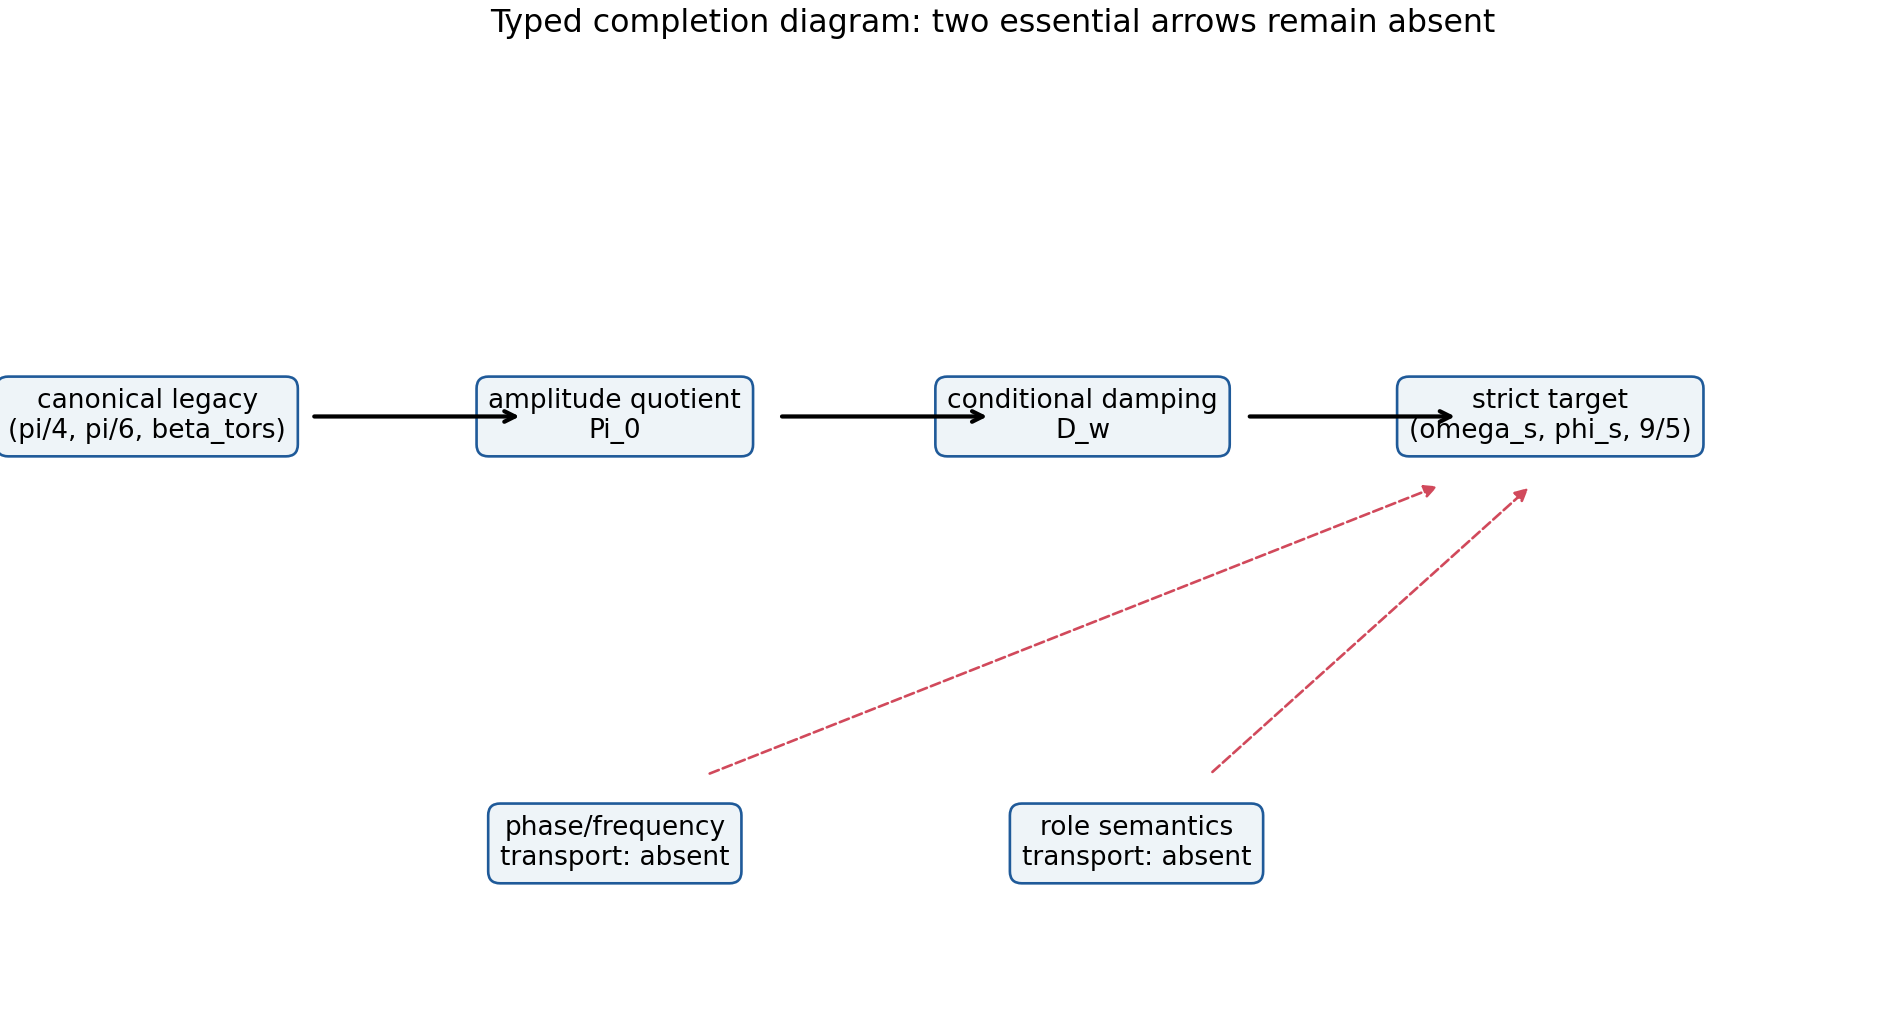
\includegraphics[width=0.94\textwidth]{FIN_Programs_138_150_State_Detector_Bridge_Figures/program149_completion_map_diagram.png}
\caption{The typed completion diagram retains absent phase/frequency and role-transfer arrows.}
\end{figure}

The typed diagram therefore has:

\begin{itemize}
\item 
a proven amplitude-quotient arrow;

\item 
a conditional damping arrow;

\item 
no phase/\allowbreak{}frequency transport arrow;

\item 
no strict selector/\allowbreak{}topological transport arrow;

\item 
no physical-role transport arrow.

\end{itemize}

\textbf{Result:} \textbf{Constructed diagram and finite noncommutation witness.}

The damping result of Programs 135 and 148 is not a full legacy-to-strict bridge. Role-transfer auditing remains downstream.

\par\medskip\hrule\medskip

\chapter{Part VI --- Program 150: an immutable pre-data physical protocol}

\section{Operational question}

The protocol asks a deliberately narrow physical question:

\begin{quote}\itshape
Does a calibrated one-dimensional spreading record behave like local diffusion with \(\alpha=2\), or like fractional spreading with \(\alpha=4/5\)?

\end{quote}

It does not attempt to test the FIN ontology, cosmology, or Theory-of- Everything claims.

\section{Frozen design}

The protocol identifier is:

FIN-P150-FRACTIONAL-IQR-001.

The design fixes:

\begin{itemize}
\item 
one documented localized preparation;

\item 
observation times \(t_1=1\) and \(t_2=4\);

\item 
at least 4,000 position records per time;

\item 
a Gaussian detector response;

\item 
known-input apparatus calibration before test records;

\item 
primary statistic

\end{itemize}

\[
T
=
\frac{
\log[\operatorname{IQR}(4)/\operatorname{IQR}(1)]
}{
\log4
};
\]

\begin{itemize}
\item 
null

\end{itemize}

\[
H_0:\alpha=2,\qquad T=\frac12;
\]

\begin{itemize}
\item 
alternative

\end{itemize}

\[
H_1:\alpha=\frac45,\qquad T=\frac54;
\]

\begin{itemize}
\item 
rejection threshold

\end{itemize}

\[
T>0.875.
\]

The canonical frozen-core digest is

0c292bf5d8efce3055a27daa16e60d60b53e2e2cb9852c37827418ec1ec453f5.

\section{Synthetic power audit}

With 450 replicates and 4,000 records per time:

\[
\begin{array}{c|cc}
&\text{mean}&\text{standard deviation}\\
\hline
H_0&0.499047&0.018354\\
H_1&1.245623&0.030951
\end{array}
\]

The declared synthetic false-positive rate is zero and synthetic power is one. These values reflect the deliberately well-separated simple hypotheses.

\begin{figure}[htbp]
\centering
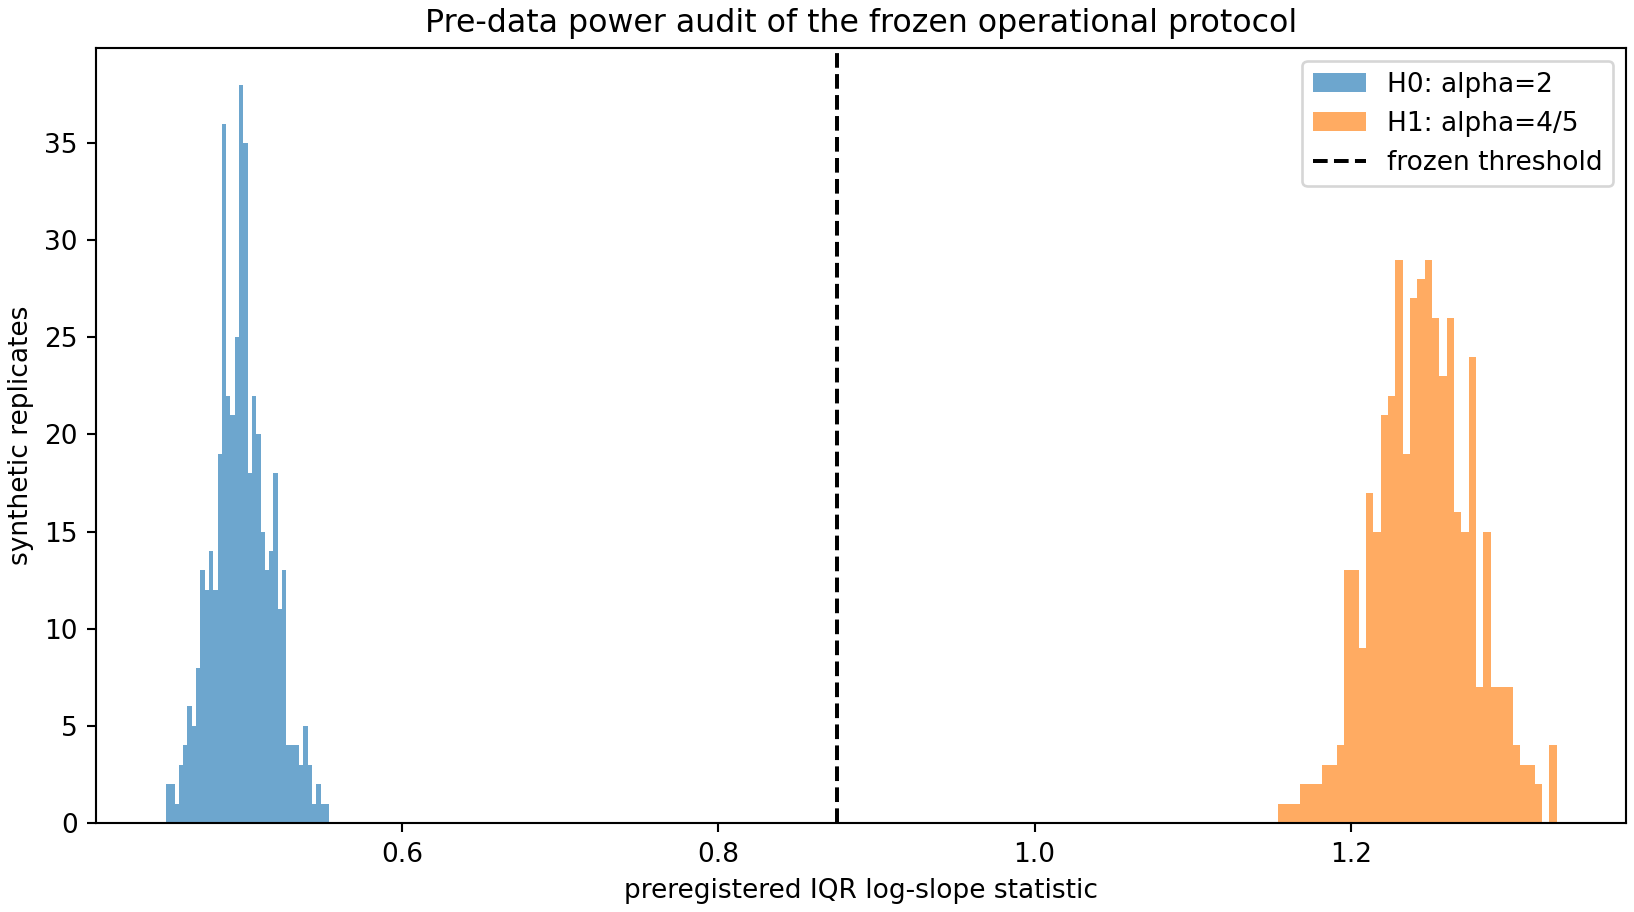
\includegraphics[width=0.94\textwidth]{FIN_Programs_138_150_State_Detector_Bridge_Figures/program150_predata_protocol_power.png}
\caption{Synthetic power audit of the immutable pre-data operational protocol.}
\end{figure}

\textbf{Result:} \textbf{Constructed immutable pre-data protocol.}

No external data have been selected or admitted. A successful future rejection would concern the declared operational models only.

\par\medskip\hrule\medskip

\chapter{Part VII --- Integrated conclusions and falsification ledger}

\section{Newly constructed objects}

The round constructs:

\begin{enumerate}
\item 
a modular/\allowbreak{}KMS state-selection no-go theorem;

\item 
a reference-measure entropy classification;

\item 
a Morita amplification trace test;

\item 
a validated interval FFT;

\item 
a finite Diophantine discrepancy modulus;

\item 
a Sobolev wave-record space;

\item 
a Gaussian detector-resolution family;

\item 
an exact joint system--instrument inverse map;

\item 
a calibration-invariant IQR observable;

\item 
a reflection-asymmetry preparation resource theory;

\item 
a strictly convex coupled state--damping action family;

\item 
a typed completion-map diagram;

\item 
an immutable pre-data physical protocol.

\end{enumerate}

\section{Falsification ledger}

\subsection{"Modular flow selects the physical state"}

\textbf{Refuted in the present finite algebra.} The commutative flow is trivial; the noncommutative modular flow is defined from a state rather than selecting it.

\subsection{"Maximum entropy forces uniform sector weights"}

\textbf{Refuted without a reference measure.} Sector counting, Hilbert counting, and Hilbert--Schmidt counting give different exponents.

\subsection{"The Hilbert trace is categorical"}

\textbf{Refuted.} Morita-equivalent block amplification changes its central weights.

\subsection{"The earlier 2.2647\% fractional bound is already formal"}

\textbf{Refuted.} The validated interval FFT supports compatibility with the fractional scale but yields the coarser formal bound \(1.08135\).

\subsection{"A finite continued fraction proves an all-scale rate"}

\textbf{Refuted.} Future partial quotients remain uncontrolled.

\subsection{"A wave detector must always have a hard UV cutoff"}

\textbf{Refined.} A regular \(H^s\), \(s>1/2\), preparation admits pointwise records without a hard cutoff. Ideal delta preparation does not.

\subsection{"Apparatus memory is inevitably confounded with the exponent"}

\textbf{Refuted in the declared three-parameter model.} Two means and one lag give an exact inverse.

\subsection{"Physical scales prevent any direct test"}

\textbf{Refuted for selected ratios.} The IQR log-slope cancels multiplicative length and time scales.

\subsection{"A signed receiver supplies the missing selector"}

\textbf{Refuted theoremically.} Its output is bounded by a preparation-asymmetry resource that free symmetric operations cannot create.

\subsection{"Amplitude plus damping completes legacy to strict"}

\textbf{Refuted for canonical legacy parameters.} The residual is \(0.470865\); phase/\allowbreak{}frequency transport is absent.

\section{Deepest surviving interpretation}

The most defensible architecture is:

\[
\begin{gathered}
\boxed{\text{dimensionless strict spectral generator}}
\\ \downarrow \\
\boxed{\text{natural localizer plus an unsourced sector state}}
\\ \downarrow \\
\boxed{\text{prepared operational process plus detector}}
\\ \downarrow \\
\boxed{\text{calibration-invariant statistics and external records}}.
\end{gathered}
\]

The first object is mathematical. The localizer is now natural. The state, signed preparation, and physical calibration remain separate interfaces. Some physical tests can cancel multiplicative calibration, but no statistic can replace the need for preparation provenance, detector modelling, and raw records.

The single most important missing theorem is now:

\begin{quote}\itshape
a non-target-coded law selecting a faithful state on the localized sector algebra and coupling it to damping.

\end{quote}

Even such a theorem would not by itself supply signed preparation or physical units. The resource theorem proves that the selector obstruction is logically independent of the sector-state obstruction.

\section{Claim table}

\subsection{Proven}

\begin{itemize}
\item 
KMS nonselection on the finite sector algebra;

\item 
reference dependence of maximum entropy;

\item 
Morita instability of the normalized Hilbert trace;

\item 
formal interval enclosure of all 50 frequency cells;

\item 
finite Denjoy--Koksma/\allowbreak{}Ostrowski discrepancy modulus;

\item 
\(H^s\), \(s>1/2\), point-record theorem;

\item 
regular detector-resolution limit;

\item 
exact inverse in the declared system--instrument model;

\item 
preparation-asymmetry monotonicity and receiver bound;

\item 
strict convexity and stationary solution of the coupled action;

\item 
noncommutation of the canonical bridge diagram.

\end{itemize}

\subsection{Strong evidence}

\begin{itemize}
\item 
finite-sample performance of joint inversion;

\item 
robustness of the IQR exponent statistic;

\item 
synthetic power of the frozen physical protocol.

\end{itemize}

\subsection{Conditional}

\begin{itemize}
\item 
\(9/5\) from sector-counting reference;

\item 
\(9/5\) from a modular gap \(\log2\);

\item 
\(\beta=1\) from positive multiplicative monomial damping;

\item 
detector-resolution removal for regular preparations;

\item 
empirical execution after apparatus and data intake.

\end{itemize}

\subsection{Open}

\begin{itemize}
\item 
a strict state/\allowbreak{}reference selection theorem;

\item 
a strict signed preparation resource;

\item 
a formal tight fractional remainder below three percent;

\item 
an all-scale Diophantine remainder rate;

\item 
phase/\allowbreak{}frequency bridge;

\item 
physical-role transfer;

\item 
internal units;

\item 
external validation.

\end{itemize}

\par\medskip\hrule\medskip

\chapter{Part VIII --- Recommended Programs 151--163}

\section{Program 151 --- Tight validated fractional certificate}

Repeat Program 141 with an Arb/\allowbreak{}FLINT-style ball FFT or a distributed interval transform at substantially larger \(N\). The acceptance target is a formal relative-remainder bound below \(3\%\) on the entire window.

\textbf{Probability of useful improvement:} 0.90.\\
\textbf{Probability of reaching \(3\%\) with available local resources:} 0.55.

\section{Program 152 --- Effective all-scale irrationality measure}

Search for a rigorous effective lower bound on

\[
\left|
\frac{743}{4000\pi}-\frac pq
\right|
\]

using explicit transcendence measures. Translate it into a discrepancy and Abelian remainder theorem. If known constants are too weak, prove that the route cannot improve practical bounds.

\textbf{Probability of a mathematically valid bound:} 0.55.\\
\textbf{Probability of a useful numerical rate:} 0.20.

\section{Program 153 --- Functorial probability measure on the fibre groupoid}

Construct the groupoid of localized fibres and all admitted isomorphisms. Classify natural probability measures on its connected components. Determine whether normalization, additivity, and induction/\allowbreak{}restriction compatibility select a unique central state.

\textbf{Probability of a classification theorem:} 0.80.\\
\textbf{Probability of selecting \(w_2=1/5\):} 0.20.

\section{Program 154 --- Carrier-sourced modular Hamiltonian}

Enumerate basis-free operators generated from \(m_p\), kernel homology, and the real-character action. Test whether any natural Hamiltonian has a unique dimensionless gap \(\log2\) without using \(\alpha_{\rm geo}/4\) as an input.

\textbf{Probability of a useful no-go theorem:} 0.75.\\
\textbf{Probability of strict state selection:} 0.15.

\section{Program 155 --- Completeness of the reflection-asymmetry resource}

Classify reflection-covariant channels on \(C_{12}\) and determine whether \(M(\rho)\) is a complete convertibility monotone for the relevant pure and mixed state families. Compute resource cost and distillation rate for signed preparation.

\textbf{Probability of a strong finite theorem:} 0.85.

\section{Program 156 --- Detector deconvolution and finite-sample bias}

Derive confidence intervals for the IQR slope under finite Gaussian resolution, correlated detector noise, censoring, and pixelization. Specify when deconvolution is identifiable and when it amplifies UV noise.

\textbf{Probability of operational success:} 0.90.

\section{Program 157 --- Semiparametric system--instrument identifiability}

Replace the three-parameter apparatus with an unknown finite-memory channel. Derive tangent-space or rank conditions separating the fractional exponent from detector dynamics. Include explicit nonidentifiable counterexamples.

\textbf{Probability of useful partial characterization:} 0.75.

\section{Program 158 --- Finite-sample theorem for the stable IQR exponent}

Derive asymptotic variance, concentration bounds, and robust confidence intervals for

\[
\widehat T
=
\frac{\log[\widehat{\operatorname{IQR}}(t_2)/
\widehat{\operatorname{IQR}}(t_1)]}{\log(t_2/t_1)}.
\]

Compare IQR, median absolute deviation, and empirical characteristic-function estimators.

\textbf{Probability of success:} 0.90.

\section{Program 159 --- Blind adversarial protocol challenge}

Generate hidden records from local, fractional, tempered-stable, truncated, and apparatus-confounded alternatives. Freeze the analysis code before labels are revealed. Measure false attribution of generic heavy tails to FIN.

\textbf{Probability of useful falsification evidence:} 0.95.

\section{Program 160 --- Phase/\allowbreak{}frequency bridge obstruction theorem}

Classify maps between the legacy period-eight oscillatory representation and the strict \(C_{12}\)/\allowbreak{}irrational-phase representation under translation, reflection, and spectral covariance. Prove either a typed transport or a representation-theoretic obstruction.

\textbf{Probability of an obstruction theorem:} 0.80.\\
\textbf{Probability of a positive canonical bridge:} 0.10.

\section{Program 161 --- Reference-exponent source grammar}

Enumerate a finite basis-free grammar for the missing \(a\) in \(r_{a,p}\propto d_p^a\). Require naturality, graph-size transfer, and a unique minimum. Charge description length and reject target-equivalent formulas.

\textbf{Probability of useful no-go:} 0.80.\\
\textbf{Probability of selecting \(a=0\):} 0.15.

\section{Program 162 --- Conditional role-transfer obstruction matrix}

Without transferring any role, determine which legacy observables are destroyed by amplitude quotient, damping completion, and phase mismatch. Produce necessary conditions that any future full bridge must satisfy before role transfer may begin.

\textbf{Probability of success:} 0.95.

\section{Program 163 --- External intake readiness audit}

Audit candidate laboratory platforms and datasets only against the frozen Program-150 schema: preparation, times, raw positions, detector calibration, memory calibration, provenance, and exclusions. Admit no dataset failing a mandatory field.

\textbf{Probability of finding a schema-compatible public dataset:} unknown.\\
\textbf{Scientific value of a zero-admission result:} high.

\section{Priority order}

The recommended order is

\[
151\to158\to156\to159\to153\to155\to160\to162\to157\to163,
\]

with Programs 152, 154, and 161 as higher-risk source-theorem branches.

The logic is:

\begin{enumerate}
\item 
make the strongest numerical theorem formally tight;

\item 
give the physical statistic a finite-sample theory;

\item 
adversarially test model specificity;

\item 
continue state and signed-resource mathematics;

\item 
attack the actual phase/\allowbreak{}frequency bridge;

\item 
admit external data only after readiness is demonstrated.

\end{enumerate}

\par\medskip\hrule\medskip

\chapter{Reproducibility statement}

The executable research file is

fin\_programs\_138\_150\_state\_detector\_bridge.py.

Machine-readable results are in

FIN\_Programs\_138\_150\_State\_Detector\_Bridge\_Results.json.

The immutable protocol is

FIN\_Programs\_138\_150\_PreData\_Physical\_Protocol.json.

Forty-two regression tests are in

test\_fin\_programs\_138\_150\_state\_detector\_bridge.py.

Thirteen figures are generated by the same executable. Synthetic calculations use seed 20260727. No external dataset is admitted.

\chapter{Conclusion}

Programs 138--150 substantially narrow the missing mathematical principle. The natural localizer does not become a physical state through KMS theory, maximum entropy, or Morita equivalence. Those frameworks organize a supplied state but do not uniquely create one in the present finite structure.

At the same time, the path from the fractional operator to an experimentally meaningful observable is shorter than before. Regular wave records, detector resolution, joint apparatus identification, calibration-invariant spreading statistics, and a pre-data protocol have all been constructed explicitly.

The selector obstruction is now also expressed as a resource theorem: reflection-symmetric free operations cannot create signed preparation. This proves that the missing sign is not recoverable merely by reading the same radial operator more cleverly.

The deepest interpretation surviving falsification is therefore:

\begin{quote}\itshape
FIN supplies a dimensionless fractional spectral generator and a natural finite informational localizer. A physical theory additionally requires a selected sector state, a nonfree preparation resource, an instrument, and calibrated records. Some calibration dependence can be removed by ratios, but the state and preparation sources remain genuinely independent mathematical obligations.

\end{quote}

\chapter{Selected references}

\begin{enumerate}
\item 
M. Takesaki, \emph{Theory of Operator Algebras I}, Springer.

\item 
O. Bratteli and D. Robinson, \emph{Operator Algebras and Quantum Statistical Mechanics}, Springer.

\item 
M. Rieffel, "Morita equivalence for operator algebras," in \emph{Operator Algebras and Applications}.

\item 
W. Feller, \emph{An Introduction to Probability Theory and Its Applications, Volume II}, Wiley.

\item 
K. Sato, \emph{Lévy Processes and Infinitely Divisible Distributions}, Cambridge University Press.

\item 
L. Kuipers and H. Niederreiter, \emph{Uniform Distribution of Sequences}, Wiley.

\item 
M. Drmota and R. Tichy, \emph{Sequences, Discrepancies and Applications}, Springer.

\item 
E. M. Stein, \emph{Singular Integrals and Differentiability Properties of Functions}, Princeton University Press.

\item 
F. Brandão and G. Gour, "Reversible framework for quantum resource theories," \emph{Physical Review Letters} 115, 070503.

\item 
A. van der Vaart, \emph{Asymptotic Statistics}, Cambridge University Press.

\end{enumerate}

\chapter{Suggested citation}

\.Zuchowski, K. (2026). \emph{FIN Programs 138--150: State Selection, Validated Fractional Dynamics, Detector Physics, and Bridge Architecture} (FIN Research Monograph, Release 10.14; Version 1.0.0) [Preprint]. Zenodo.


\clearpage
\chapter*{Archival note}
\addcontentsline{toc}{chapter}{Archival note}
Machine-readable results are stored in
\path{FIN_Programs_138_150_State_Detector_Bridge_Results.json}.
The executable, forty-two tests, thirteen figures, and immutable pre-data
protocol reproduce the release.

\medskip
\noindent\textbf{Suggested citation:}

\.Zuchowski, K. (2026). \emph{FIN Programs 138--150: State Selection,
Validated Fractional Dynamics, Detector Physics, and Bridge Architecture}
(FIN Research Monograph, Release 10.14; Version 1.0.0) [Preprint]. Zenodo.
\end{document}
